% Options for packages loaded elsewhere
\PassOptionsToPackage{unicode}{hyperref}
\PassOptionsToPackage{hyphens}{url}
\documentclass[
]{article}
\usepackage{xcolor}
\usepackage{amsmath,amssymb}
\setcounter{secnumdepth}{-\maxdimen} % remove section numbering
\usepackage{iftex}
\ifPDFTeX
  \usepackage[T1]{fontenc}
  \usepackage[utf8]{inputenc}
  \usepackage{textcomp} % provide euro and other symbols
\else % if luatex or xetex
  \usepackage{unicode-math} % this also loads fontspec
  \defaultfontfeatures{Scale=MatchLowercase}
  \defaultfontfeatures[\rmfamily]{Ligatures=TeX,Scale=1}
\fi
\usepackage{lmodern}
\ifPDFTeX\else
  % xetex/luatex font selection
\fi
% Use upquote if available, for straight quotes in verbatim environments
\IfFileExists{upquote.sty}{\usepackage{upquote}}{}
\IfFileExists{microtype.sty}{% use microtype if available
  \usepackage[]{microtype}
  \UseMicrotypeSet[protrusion]{basicmath} % disable protrusion for tt fonts
}{}
\makeatletter
\@ifundefined{KOMAClassName}{% if non-KOMA class
  \IfFileExists{parskip.sty}{%
    \usepackage{parskip}
  }{% else
    \setlength{\parindent}{0pt}
    \setlength{\parskip}{6pt plus 2pt minus 1pt}}
}{% if KOMA class
  \KOMAoptions{parskip=half}}
\makeatother
\usepackage{longtable,booktabs,array}
\newcounter{none} % for unnumbered tables
\usepackage{calc} % for calculating minipage widths
% Correct order of tables after \paragraph or \subparagraph
\usepackage{etoolbox}
\makeatletter
\patchcmd\longtable{\par}{\if@noskipsec\mbox{}\fi\par}{}{}
\makeatother
% Allow footnotes in longtable head/foot
\IfFileExists{footnotehyper.sty}{\usepackage{footnotehyper}}{\usepackage{footnote}}
\makesavenoteenv{longtable}
\usepackage{graphicx}
\makeatletter
\newsavebox\pandoc@box
\newcommand*\pandocbounded[1]{% scales image to fit in text height/width
  \sbox\pandoc@box{#1}%
  \Gscale@div\@tempa{\textheight}{\dimexpr\ht\pandoc@box+\dp\pandoc@box\relax}%
  \Gscale@div\@tempb{\linewidth}{\wd\pandoc@box}%
  \ifdim\@tempb\p@<\@tempa\p@\let\@tempa\@tempb\fi% select the smaller of both
  \ifdim\@tempa\p@<\p@\scalebox{\@tempa}{\usebox\pandoc@box}%
  \else\usebox{\pandoc@box}%
  \fi%
}
% Set default figure placement to htbp
\def\fps@figure{htbp}
\makeatother
\ifLuaTeX
  \usepackage{luacolor}
  \usepackage[soul]{lua-ul}
\else
  \usepackage{soul}
\fi
\setlength{\emergencystretch}{3em} % prevent overfull lines
\providecommand{\tightlist}{%
  \setlength{\itemsep}{0pt}\setlength{\parskip}{0pt}}
\usepackage{bookmark}
\IfFileExists{xurl.sty}{\usepackage{xurl}}{} % add URL line breaks if available
\urlstyle{same}
\hypersetup{
  hidelinks,
  pdfcreator={LaTeX via pandoc}}

\author{}
\date{}

\begin{document}

{\def\LTcaptype{none} % do not increment counter
\begin{longtable}[]{@{}
  >{\raggedright\arraybackslash}p{(\linewidth - 2\tabcolsep) * \real{0.1358}}
  >{\raggedright\arraybackslash}p{(\linewidth - 2\tabcolsep) * \real{0.8312}}@{}}
\toprule\noalign{}
\endhead
\bottomrule\noalign{}
\endlastfoot
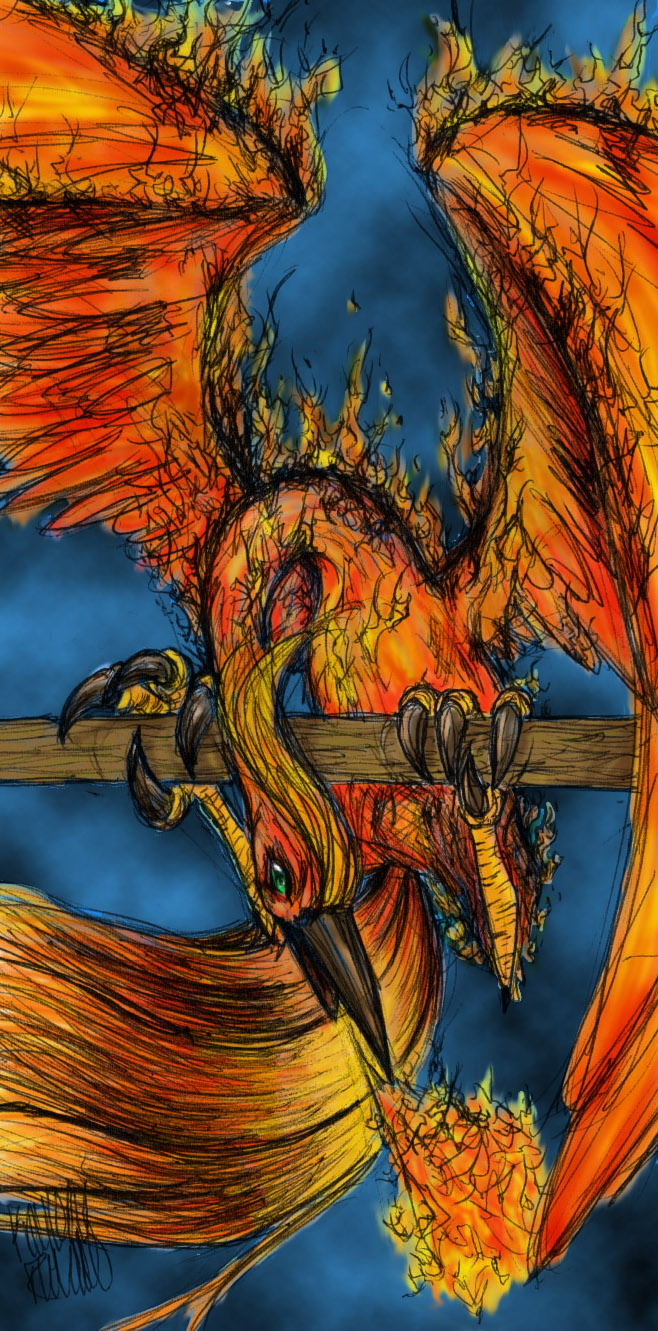
\includegraphics[width=3.35333in,height=9.8066in,alt={M:\textbackslash My Pictures\textbackslash Drawing Scans\textbackslash pheonixcoloured.JPG}]{./images/media/image1.jpeg} & \begin{minipage}[t]{\linewidth}\raggedright
\begin{quote}
\emph{\textbf{XDD}}

\emph{\textbf{User Guide}}
\end{quote}
\end{minipage} \\
\end{longtable}
}

\begin{quote}
Version 7.0.0.rc21-1

April 2012

I/O Performance, Inc.

Copyright © 1992-2012, I/O Performance, Inc.
\end{quote}

{\def\LTcaptype{none} % do not increment counter
\begin{longtable}[]{@{}
  >{\raggedright\arraybackslash}p{(\linewidth - 4\tabcolsep) * \real{0.2433}}
  >{\raggedright\arraybackslash}p{(\linewidth - 4\tabcolsep) * \real{0.0268}}
  >{\raggedright\arraybackslash}p{(\linewidth - 4\tabcolsep) * \real{0.3668}}@{}}
\toprule\noalign{}
\endhead
\bottomrule\noalign{}
\endlastfoot
\multicolumn{2}{@{}>{\raggedright\arraybackslash}p{(\linewidth - 4\tabcolsep) * \real{0.2702} + 2\tabcolsep}}{%
Principle Author:

Contributing Authors:} & Thomas M. Ruwart

\emph{tmruwart@ioperformance.com}

Steve Hodson, DoE/ORNL

\emph{hodsonsw@ornl.gov}

Steve Poole, DoE/ORNL

\emph{spoole@ornl.gov}

Bradly Settlemyer, DoE/ORNL

\emph{settlemyerbw@ornl.gov}

Russell Cattelan, Digital Elves

\emph{russell@thebarn.com}

Alex Elder \\
\multicolumn{2}{@{}>{\raggedright\arraybackslash}p{(\linewidth - 4\tabcolsep) * \real{0.2702} + 2\tabcolsep}}{%
} & \\
\multicolumn{2}{@{}>{\raggedright\arraybackslash}p{(\linewidth - 4\tabcolsep) * \real{0.2702} + 2\tabcolsep}}{%
Phone:} & 612-850-2918 \\
\multicolumn{2}{@{}>{\raggedright\arraybackslash}p{(\linewidth - 4\tabcolsep) * \real{0.2702} + 2\tabcolsep}}{%
Email:} & tmruwart@ioperformance.com \\
& \multicolumn{2}{>{\raggedright\arraybackslash}p{(\linewidth - 4\tabcolsep) * \real{0.3936} + 2\tabcolsep}@{}}{%
} \\
\end{longtable}
}

\textbf{Change History:}

The revision numbers have the following meaning. The ``number'' such as 5.7, 5.8, 5.9, \ldots etc. represent major release changes such as the addition of new options or sections to XDD.

{\def\LTcaptype{none} % do not increment counter
\begin{longtable}[]{@{}
  >{\raggedright\arraybackslash}p{(\linewidth - 6\tabcolsep) * \real{0.1701}}
  >{\raggedright\arraybackslash}p{(\linewidth - 6\tabcolsep) * \real{0.1612}}
  >{\raggedright\arraybackslash}p{(\linewidth - 6\tabcolsep) * \real{0.2091}}
  >{\raggedright\arraybackslash}p{(\linewidth - 6\tabcolsep) * \real{0.4232}}@{}}
\toprule\noalign{}
\endhead
\bottomrule\noalign{}
\endlastfoot
Revision & Date & Author & Description of Changes \\
7.0 & 18 JAN 2010 & Thomas M. Ruwart & Release of 7.0 \\
7.0 & 01FEB2011 & Thomas M. Ruwart & Pre-release 19 of 7.1 \\
7.0 & 07APR2011 & Thomas M. Ruwart & After release of Version 7.0 rc19 \\
7.0 & 18APR2011 & Thomas M. Ruwart & New heartbeat suboptions \\
7.0 rc21-1 & 02APR2012 & Thomas M. Ruwart & Maintenance Release \\
\end{longtable}
}


\section{Table of Contents}\label{table-of-contents}

\hyperref[introduction]{1 Introduction \hyperref[introduction]{5}}

\hyperref[about-this-document]{1.1 About this document \hyperref[about-this-document]{5}}

\hyperref[acknowledgements]{1.2 Acknowledgements \hyperref[acknowledgements]{5}}

\hyperref[about-xdd]{1.3 About XDD \hyperref[about-xdd]{5}}

\hyperref[license-agreement]{1.4 License Agreement \hyperref[license-agreement]{5}}

\hyperref[distribution-of-xdd]{1.5 Distribution of XDD \hyperref[distribution-of-xdd]{5}}

\hyperref[versioning]{1.6 Versioning \hyperref[versioning]{5}}

\hyperref[system-requirements]{1.7 System Requirements \hyperref[system-requirements]{5}}

\hyperref[whats-new]{2 What's new \hyperref[whats-new]{7}}

\hyperref[in-release-7.0.0]{2.1 In Release 7.0.0 \hyperref[in-release-7.0.0]{7}}

\hyperref[compiling-and-installing-xdd]{3 Compiling and Installing XDD \hyperref[compiling-and-installing-xdd]{7}}

\hyperref[xdd-source-code-overview]{3.1 XDD Source Code Overview \hyperref[xdd-source-code-overview]{7}}

\hyperref[build-notes]{3.2 Build Notes \hyperref[build-notes]{8}}

\hyperref[configure-and-make]{3.2.1 Configure and Make \hyperref[configure-and-make]{8}}

\hyperref[supported-operating-systems]{3.2.2 Supported Operating Systems \hyperref[supported-operating-systems]{9}}

\hyperref[theory-of-operation]{4 Theory of Operation \hyperref[theory-of-operation]{10}}

\hyperref[xdd-program-structure-overview]{4.1 XDD Program Structure Overview \hyperref[xdd-program-structure-overview]{10}}

\hyperref[basic-operation]{4.2 Basic Operation \hyperref[basic-operation]{11}}

\hyperref[command-line-options-and-the-setup-file]{4.3 Command Line Options and the Setup File \hyperref[command-line-options-and-the-setup-file]{11}}

\hyperref[operation-specification]{4.4 Operation Specification \hyperref[operation-specification]{12}}

\hyperref[target-specification-and-multiple-target-synchronization]{4.5 Target Specification and Multiple Target Synchronization \hyperref[target-specification-and-multiple-target-synchronization]{12}}

\hyperref[time-synchronization-across-multiple-computer-systems]{4.6 Time Synchronization Across Multiple Computer Systems \hyperref[time-synchronization-across-multiple-computer-systems]{12}}

\hyperref[xdd-run-time-or-run-length]{4.7 XDD Run Time or Run Length \hyperref[xdd-run-time-or-run-length]{13}}

\hyperref[io-range]{4.8 I/O Range \hyperref[io-range]{14}}

\hyperref[access-patterns]{4.9 Access Patterns \hyperref[access-patterns]{15}}

\hyperref[reading-and-writing-devices-and-files]{4.10 Reading and Writing Devices and Files \hyperref[reading-and-writing-devices-and-files]{15}}

\hyperref[processor-allocation-and-priority-assignment]{4.11 Processor Allocation and Priority Assignment \hyperref[processor-allocation-and-priority-assignment]{17}}

\hyperref[preallocation]{4.12 Preallocation \hyperref[preallocation]{17}}

\hyperref[io-time-stamping]{4.13 I/O Time Stamping \hyperref[io-time-stamping]{18}}

\hyperref[running-xdd-programs]{5 Running XDD Programs \hyperref[running-xdd-programs]{20}}

\hyperref[xdd-command-line-arguments-synopsis]{5.1 XDD Command Line Arguments Synopsis \hyperref[xdd-command-line-arguments-synopsis]{20}}

\hyperref[detailed-option-specifications]{5.2 Detailed Option Specifications \hyperref[detailed-option-specifications]{23}}

\hyperref[target-specific-options]{5.3 Target-specific options \hyperref[target-specific-options]{33}}

\hyperref[lockstep-operations]{5.4 Lockstep Operations \hyperref[lockstep-operations]{33}}

\hyperref[timeserver-and-gettime]{5.5 Timeserver and gettime \hyperref[timeserver-and-gettime]{34}}

\hyperref[deskew]{5.6 Deskew \hyperref[deskew]{34}}

\hyperref[io-operation-ordering]{5.7 I/O Operation Ordering \hyperref[io-operation-ordering]{35}}

\hyperref[serial-ordering]{5.7.1 Serial Ordering \hyperref[serial-ordering]{36}}

\hyperref[loose-ordering]{5.7.2 Loose Ordering \hyperref[loose-ordering]{36}}

\hyperref[no-ordering]{5.7.3 No Ordering \hyperref[no-ordering]{37}}

\hyperref[xddcp]{6 XDDCP \hyperref[xddcp]{38}}

\hyperref[xddcp-usage]{6.1 XDDCP Usage \hyperref[xddcp-usage]{39}}

\hyperref[end-to-end-and-xddcp-theory-of-operation]{6.2 End-to-End and XDDCP Theory of Operation \hyperref[end-to-end-and-xddcp-theory-of-operation]{40}}

\hyperref[runtime-hints]{7 Runtime Hints \hyperref[runtime-hints]{42}}

\hyperref[windows]{7.1 Windows \hyperref[windows]{42}}

\hyperref[linux-1]{7.2 Linux \hyperref[linux-1]{42}}

\hyperref[freebsd]{7.3 FreeBSD \hyperref[freebsd]{42}}

\hyperref[osx]{7.4 OSX \hyperref[osx]{42}}

\hyperref[solaris]{7.5 Solaris \hyperref[solaris]{42}}

\hyperref[irix]{7.6 IRIX \hyperref[irix]{42}}

\hyperref[aix-1]{7.7 AIX \hyperref[aix-1]{43}}

\hyperref[output-and-reports]{8 Output and Reports \hyperref[output-and-reports]{44}}

\hyperref[reporting-options]{8.1 Reporting Options \hyperref[reporting-options]{44}}

\hyperref[output-format]{8.2 Output Format \hyperref[output-format]{44}}

\hyperref[what-the-numbers-really-mean]{8.3 What the numbers really mean \hyperref[what-the-numbers-really-mean]{50}}

\hyperref[performance-tuning-hints]{9 Performance Tuning Hints \hyperref[performance-tuning-hints]{51}}

\hyperref[caches-and-write-performance]{9.1 Caches and write performance \hyperref[caches-and-write-performance]{51}}

\hyperref[fibre-channel-frame-sizes]{9.2 Fibre Channel Frame Sizes \hyperref[fibre-channel-frame-sizes]{51}}

\hyperref[examples]{10 Examples \hyperref[examples]{52}}

\hyperref[example-1-basic-xdd-command-line]{10.1 Example 1 -- Basic XDD command line \hyperref[example-1-basic-xdd-command-line]{52}}

\hyperref[example-2-specifying-multiple-targets-and-timelimit]{10.2 Example 2 -- Specifying multiple targets and timelimit \hyperref[example-2-specifying-multiple-targets-and-timelimit]{52}}

\hyperref[example-3-time-stamping-and-setup-file]{10.3 Example 3 -- Time Stamping and Setup File \hyperref[example-3-time-stamping-and-setup-file]{52}}

\hyperref[example-4-random-seeks]{10.4 Example 4 -- Random Seeks \hyperref[example-4-random-seeks]{52}}

\hyperref[example-5-end-to-end-operation]{10.5 Example 5 -- End to End operation \hyperref[example-5-end-to-end-operation]{54}}

\hyperref[e2e-example-with-multiple-network-interfaces]{10.6 E2E Example with multiple Network Interfaces \hyperref[e2e-example-with-multiple-network-interfaces]{55}}

\hyperref[example-time-stamp-output]{10.7 Example Time Stamp Output \hyperref[example-time-stamp-output]{56}}

\hyperref[under-the-hood]{Under the Hood \hyperref[under-the-hood]{59}}

\hyperref[xdd-general-operation]{10.8 XDD general operation \hyperref[xdd-general-operation]{60}}

\hyperref[the-xdd-buffer-memory-layout]{10.9 The XDD buffer memory layout \hyperref[the-xdd-buffer-memory-layout]{60}}

\hyperref[the-xdd-thread-structure]{10.10 The XDD thread structure \hyperref[the-xdd-thread-structure]{61}}

\hyperref[xdd-barriers]{10.11 XDD barriers \hyperref[xdd-barriers]{61}}

\hyperref[the-gnu-public-license]{11 The GNU Public License \hyperref[the-gnu-public-license]{63}}

\hyperref[_Toc290917472]{11.1 Preamble \hyperref[_Toc290917472]{63}}

\hyperref[_Toc290917473]{11.2 TERMS AND CONDITIONS FOR COPYING, DISTRIBUTION AND MODIFICATION \hyperref[_Toc290917473]{63}}

\hyperref[no-warranty]{11.3 NO WARRANTY \hyperref[no-warranty]{64}}

\hyperref[acknowledgements-1]{12 Acknowledgements \hyperref[acknowledgements-1]{64}}

\newpage
\section{Introduction}\label{introduction}

\subsection{About this document}\label{about-this-document}

This document is a guide to compiling, installing, and running the XDD program. It also has a variety of examples and hints for understanding the use and results of XDD.

\subsection{\texorpdfstring{Acknowledgements }{Acknowledgements }}\label{acknowledgements}

The continuing work on XDD is supported by funding and resources of the National Center for Computational Sciences (NCCS) at Oak Ridge National Laboratory (ORNL), the Extreme Scale Systems Center (ESSC) at ORNL, and the Department of Defense.

\subsection{About XDD}\label{about-xdd}

XDD was originally developed in 1992 as a command-line tool for measuring performance and characterizing disk subsystem I/O behavior on anything from a single system to a large cluster of systems -- something a little bit better than the traditional ``dd'' utility in UNIX. The goal was to provide consistent and reproducible performance measurements of disk I/O traffic. After its success in the SGI IRIX\footnote{As of release 7.0.0 the IRIX Operating System is no longer supported.} environment where it was originally developed, it and has been ported to run under Linux, AIX, Solaris, MacOS X, and Windows.

Over the years XDD has assumed many capabilities. As of XDD Release 7.0 it is possible to use XDD to reliably copy exceedingly large files from one computer to another over a network at speeds approaching the capability of the underlying hardware. See the End-to-End option and examples for more information on this feature.

\subsection{License Agreement}\label{license-agreement}

It is distributed in the hope that it will be useful, but WITHOUT ANY WARRANTY; without even the implied warranty of MERCHANTABILITY or FITNESS FOR A PARTICULAR PURPOSE. See the GNU General Public License for more details. You should have received a copy of the GNU General Public License along with this program/document in a file named \textquotesingle Copying\textquotesingle{} or `gpl.txt' or in the section entitled \emph{The GNU Public License} in this document; if not, write to the Free Software Foundation, Inc., 675 Mass Ave, Cambridge, MA 02139 or visit their web site at \url{http://www.gnu.org/licenses/gpl.html}.

\subsection{Distribution of XDD}\label{distribution-of-xdd}

This program is free software; you can redistribute it and/or modify it under the terms of the GNU General Public License as published by the Free Software Foundation; either version 2 of the License, or (at your option) any later version.

\subsection{Versioning}\label{versioning}

The version numbering format is as follows:

\begin{quote}
Major.Minor.Revision-Build
\end{quote}

Where the Major and Minor are numbers (i.e. 7.0).

The Revision-Build indicate the state of the Major.Minor revision. For example, ``rc19-pre'' indicates Release Candidate number 19, with a pre-build'' status -- not a final build.

A final release distribution file would look like so:

\begin{quote}
\textbf{XDD.Linux.7.0.Build-1504.tgz}
\end{quote}

\subsection{System Requirements}\label{system-requirements}

XDD can run on a relatively minimally configured system but it is recommended that adequate main memory capacity and processor speed be available when using some of the more advanced features of XDD. The XDD program itself is not CPU intensive but the faster the processor and the less loaded a system is the more accurate and consistent the results will be. As a rule, a minimum of 128MB of main memory is recommended just for the XDD program itself. All other system parameters are left to the discretion of the user.

\newpage
\section{\texorpdfstring{What's new }{What's new }}\label{whats-new}

\subsection{In Release 7.0.0}\label{in-release-7.0.0}

There are several major changes in release 7.0 that include:

\begin{itemize}
\item
  Major restructuring of the source code for readability, extensibility, and supportability
\item
  Addition of an end-to-end option that allows XDD to quickly and reliably copy data from one computer system to another while measuring the end-to-end performance of the operation (\textbf{-endtoend} option)
\item
  A ``restart'' monitor used in conjunction with the end-to-end operations to resume a failed copy operation
\item
  Enhanced heart beat options
\item
  A ``results'' manager thread that is used to collect and display results from all I/O threads
\item
  The ability to selectively reformat the output fields (\textbf{-outputformat} option)
\item
  Ability to specify the exact number of bytes to transfer (\textbf{-bytes} option)
\item
  I/O Operation Ordering is more tightly controlled and can be specified as serial, loose, or none. See section on I/O Operation Ordering for more details.
\end{itemize}

\newpage
\section{Compiling and Installing XDD}\label{compiling-and-installing-xdd}

\subsection{XDD Source Code Overview}\label{xdd-source-code-overview}

The XDD distribution comes with all the source code necessary to install XDD and the companion programs timeserver and the gettime. For UNIX systems, a \emph{make} file is used to build any of these programs. The XDD distribution directory hierarchy has the following structure:

\subsection{Build Notes}\label{build-notes}

\subsubsection{Configure and Make}\label{configure-and-make}

The process has been simplified for most XDD-supported operating systems.

From the directory that contains the script called ``configure'' run the following command:

\begin{quote}
./configure
\end{quote}

This will build the file called ``Makefile'' that contains all the OS-dependencies adjusted for the build.

At that point run any of the following:

\begin{quote}
make
\end{quote}

or

\begin{quote}
make install
\end{quote}

or

\begin{quote}
make clean ; make
\end{quote}

A simple ``make'' will simply make the xdd, timeserver, and gettime executables in the local XDD bin subdirectory.

The ``make install'' will attempt to copy the XDD, timeserver, and gettime executables into /sbin on the local system. The user must have root privileges in order to perform a ``make install''.

The ``make clean'' is used to remove all object files and previously compiled executables from the local XDD bin directory. It must be followed by an explicit ``make'' or ``make install'' to recompile the executables.

\subsubsection{Supported Operating Systems}\label{supported-operating-systems}

XDD is currently supported on a number of mainstream operating systems with limited support for some legacy operating systems. These operating systems include:

\begin{itemize}
\item
  Linux (kernel versions 2.6 and above only)
\item
  AIX™ from IBM
\item
  Soon to be supported:

  \begin{itemize}
  \item
    Mac OS X
  \item
    FreeBSD
  \item
    Solaris™ from Sun on Intel platforms
  \item
    Windows™ NT™ , Windows™ 2000™, Windows™ XP™, Windows™ Vista™, Windows™ Server™ 2003™, Windows™ Server™ 2008™, Windows™ 7™
  \end{itemize}
\end{itemize}

The process for building XDD is relatively straight forward for all operating systems. There are two basic build environments: Windows™ systems and Unix-like systems. The basic process of building XDD is to extract the files from the XDD distribution archive and run the build program. The build program for Unix-like systems is ``make'' plus the ``c'' or ``gcc'' compiler. In either case, the XDD, timeserver, and gettime executables are built and placed in the ``bin'' subdirectory (see diagram).

For all Unix-like systems that there will be an executable with and without the operating system name as an extension. For example, on a Linux system, the build process will produce an executable file called ``xdd.Linux'' and one called ``XDD''. The ``XDD'' executable is simply a hard link to the ``xdd.Linux'' executable. The same applies to the ``timeserver'' and ``gettime'' executable files.

Finally, it is important to note that XDD does not depend on the ``timeserver'' or ``gettime'' programs. These additional programs are used in multi-hosted environments.

\paragraph{Linux}\label{linux}

Make uses either the cc or gcc compiler and associated libraries. Insure that the pthreads libraries are installed for correct compilation and linking. This is normally the case for most modern Linux installations.

At the successful conclusion of the build process, the ``bin'' directory will contain the following files:

\begin{itemize}
\item
  ``xdd.Linux'' and a hard link to ``xdd''
\item
  ``timeserver.Linux'' and a hard link to ``timeserver''
\item
  ``gettime.Linux'' and a hard link to ``gettime''
\end{itemize}

\paragraph{AIX}\label{aix}

As in Linux, ensure that the \ul{pthread} libraries are installed.

\newpage
\section{Theory of Operation}\label{theory-of-operation}

\subsection{XDD Program Structure Overview}\label{xdd-program-structure-overview}

XDD consists of the main XDD executable and one or more ``target'' threads that are created to perform the actual I/O operations on a specific target device or file. The following terms are important to understand in order to make sense of the program and source code structure:

\begin{itemize}
\item
  The time from the invocation of the XDD command until it returns control to the shell is referred to as a ``run''
\item
  Each ``run'' consists of one or more ``passes''
\item
  Each ``pass'' consists of one or more I/O ``operations''
\end{itemize}

For example, the following simple XDD command line will perform an XDD ``run'' that consists 5 passes of 128 write I/O Operations (4Kbytes each) to be performed on the specified ``target'' called ``testfile''. The ``verbose'' option will cause XDD to display intermediate results for each ``pass'' as the pass completes.

\begin{quote}
\textbf{XDD --op write --target testfile -blocksize 4 --numreqs 128 --passes 5 --verbose}
\end{quote}

The overall program structure has been simplified the several basic parts as shown:

\emph{QThread}

target\_pass subroutine

Target Thread

\subsection{Basic Operation}\label{basic-operation}

XDD is a program that performs data transfer operations between memory and a disk device or file (or multiple disk devices / files) and collects and displays performance information about these I/O operations. XDD creates one Target Thread for every device or file under test. Each XDD Target Thread creates one or more QThreads (aka ``worker'' threads) and issues ``tasks'' to available QThreads to perform required. A QThread given an I/O task will issue an I/O operation to the ``target'' which is either a disk storage device or a file. Each I/O operation is either a read or a write operation of a fixed multiple of the "block size". Optionally, the QThread will also perform a ``send'' or ``receive'' operation to a network ``socket'' if the End-to-End option had been specified.

An XDD ``run'' consists of several ``passes'', the number of which is specified by the ``--passes'' option. Each pass will execute some number of I/O requests on the specified target(s) at the given block size. In general, each pass is identical to the previous passes in a run with respect to the block size, number of requests to issue, and the access pattern unless certain options are used to alter these parameters between passes. Passes are run one after another with no delays between passes unless a pass delay is specified with the ``--delay'' option.

Multiple passes within an XDD run are used to determine the reproducibility of the results. In theory, the results from each pass in an XDD run should be the same or at least very close to the same given the same set of run-time parameters.

Upon invocation, XDD will parse the command line arguments and spawn one Target Thread for each target specified for the run. The Target Thread will spawn additional ``QThreads'' according to the ``-queuedepth'' option. After the Target Threads have been initialized they will wait at an ``initialization barrier'' until XDD ``main'' has spawned and initialized the Results Manager thread and optionally the Heartbeat and/or the Restart Monitor threads which depend on the --heartbeat and --restart options respectively.

\subsection{Command Line Options and the Setup File}\label{command-line-options-and-the-setup-file}

XDD has a command-line interface that requires all the run-time parameters to be specified either on the XDD invocation command line or in a ``setup'' file. The format of the setup file is similar to the XDD command-line in that the options can be simply entered into the setup file the same as they would be seen on the command line. The following example shows an XDD invocation using just the command-line and the same invocation using the setup file along with the contents of the setup file.

Command line:

\begin{quote}
xdd --op read --targets 1 /dev/scsi/disk1 --blocksize 8 --numreqs 128

--verbose
\end{quote}

Using a Setup file:

xdd --setup XDDrun.txt

--op read --targets 1 /dev/scsi/disk1

--blocksize 8

--numreqs 128

--verbose

Where the setup file XDDrun.txt is an ASCII text file that contains the following:

\subsection{Operation Specification}\label{operation-specification}

The operation to perform is specified by the ``--\textbf{op}'' option. This can be either ``\emph{read}'' or ``\emph{write}''. This version of XDD \emph{will} mix read and write operations within an XDD run according to the read/write ratio set using the \textbf{--rwratio} option. Each r/w operation will transfer a given amount of data known as the ``block size''. A block is, by default, 4096 bytes but can be specified to be any positive integer value by using the ``--\textbf{blocksize}'' option. The ``block'' is used as the basic unit for all other options requiring a data size unless otherwise noted. It is recommended that the block size be specified as numbers that are integer multiples of 512 bytes (i.e. 1024, 2048, 5120, \ldots etc.) since this tends to be the predominant sector size for most storage devices at the current time.

\subsection{Target Specification and Multiple Target Synchronization}\label{target-specification-and-multiple-target-synchronization}

All requests are sent to a ``target'' which can be either a disk device or a file. A single XDD run can operate on a single target or multiple targets simultaneously. Target names are specified using the ``--\textbf{targets}'' option. It is always necessary to specify the number of targets followed by the individual target names. In order to simplify the list of target names, the ``-\textbf{targetdir}'' option can be used to specify the directory where the target devices or files reside.

The execution of the XDD threads on multiple targets is synchronized through the use of "barriers". Each XDD Target Thread initializes itself and waits for all the other XDD Target Threads to "reach at starting point". Once all the XDD Target Threads reach this point, they are all released simultaneously. Each XDD Target Thread will run independently until it has either completed all of its requested I/O operations or reached its time limit (as specified by the --\textbf{timelimit} input parameter). At this point the XDD Target Threads synchronize with the Results Manager Thread that will collect and display the intermediate results for the pass that just completed. After displaying the results the Target Threads will be released to begin another pass or to perform their end-of-run processing.

It is also possible to resynchronize the Target Threads at specific points within a pass by using the ``--\textbf{syncio}'' and/or ``-\textbf{syncwrite}'' options. The -\textbf{syncio} option instructs each of the Target Threads to synchronize after some number of I/O operations specified as an argument to this option. The default is to synchronize only at the beginning of each pass. The --\textbf{syncwrite} option is used to synchronize ``buffered'' write operations at the end of each pass by flushing all the file system data buffers to the physical media. This option is not able to flush and cache buffers on the disk controllers or disk drives themselves.

Synchronizing the XDD Target Threads is done to insure that all the XDD Target Threads start at precisely the same time in order to avoid misleading results due to skewing the start times. It is possible to eliminate synchronization by specifying the -\textbf{nobarrier} parameter. The result is that many of the I/O start times can be significantly skewed from one another for all participating XDD Target Threads. However, that may in fact be the desired effect.

\subsection{Time Synchronization Across Multiple Computer Systems}\label{time-synchronization-across-multiple-computer-systems}

Synchronization can also be done across multiple machines each running XDD. This is accomplished by using the timeserver and gettime programs. The timeserver program provides a single global reference clock that is used by the time stamping in order to be able to more accurately correlate events in time from multiple computer systems. The timeserver program should be run on a single machine as a background task. This machine must be accessible via a LAN to all the machines that will be running XDD. This LAN should preferably be a lightly used LAN for optimum results.

The preferred way to make this work is to use ``ssh'' to start the XDD programs on each of the nodes using the ``-starttime'' and ``-timeserver'' options. The ``-timeserver'' option tells the XDD program the host name or IP address of the timeserver machine. The XDD program will contact this machine to determine the ``global'' time that all the other XDD programs will use as a frame of reference. The ``-starttime'' option specifies the time to start in ``global time'' units.

Before running the ``ssh XDD'' command line in a script, it is necessary to determine a global time sometime in the future at which all the XDD program will start. The way to do this is to use the ``gettime'' program to contact the time server, determine the global time, add a specified number of seconds, and display the result on standard out. This global start time can then be used as the argument to the ``-starttime'' option for each of the ``rsh XDD'' commands. An example script would look like so:

\begin{quote}
\ldots.

set g=`gettime --timeserver 192.10.11.12 --add 20`

\# At this point \$\{g\} will be the current global time plus

\# 20 seconds.

foreach i ( 1 2 3 4 )

ssh host\$\{i\} XDD --starttime \$\{g\} --op read --targets 1 /dev/dsk/c1d2s0 --mbytes 5 --timeserver host 192.10.11.12 \ldots\&

end

wait

\ldots{}
\end{quote}

This example scriptlet will set the local variable ``\$\{g\}'' to the global time plus 20 seconds. This value is then passed to each of the XDD programs that are started on host1, host2, host3, and host4. This will result in each XDD program starting at exactly the same time. However, if any or all of the host machines running XDD are in the presence of a black hole, neutron star, or other extremely massive body, the relativistic effects on the space-time continuum may produce unpredictable results.

\subsection{XDD Run Time or Run Length}\label{xdd-run-time-or-run-length}

It is necessary to specify a limit on how \emph{long} XDD will run. There are several ways to do this. First, it is possible to explicitly specify the number of transfers to perform using the ``--\textbf{numreqs}'' option. This specifies the number of read or write calls to make for a single ``pass''. It is also possible to simply specify the number of MegaBytes to transfer using the ``--\textbf{bytes}'', ``--\textbf{kbytes}'', ``--\textbf{mbytes}'', or ``--\textbf{gbytes}'', option. It is important to note that a KiloByte, MegaByte, GigaByte in this context is a power of two: 1024, 1048576, or 1073741824 bytes. Finally, it is possible to specify a time limit for each XDD pass using the --\textbf{timelimit} option. This will cause each pass to terminate after the specified number of seconds has elapsed or after executing the specified number of requests or transferring the specified number of megabytes whichever occurs first.

\subsection{I/O Range}\label{io-range}

For random I/O operations, each XDD I/O thread performs its I/O operations within a certain consecutive ``range'' of blocks on the target (see Figure 1). The range is either \emph{implicitly} specified as the number of MegaBytes to transfer or \emph{explicitly} specified using the ``--\textbf{range}'' option. For example, if the user specifies ``2048k'' bytes in data transfers, then the range will be implied as 512 blocks (512 * 4096). However, if the user wants to transfer the same 2048k bytes randomly over a 2 GigaByte area (or range) on the target then the range needs to be explicitly specified as 512 requests or 2 GigaBytes.

The beginning of the I/O range defaults to the beginning of the target whether it is a device or a file. It is possible to specify a ``starting offset'' such that the I/O range begins at some distance into the target (see Figure 1). This can be done several ways. First, the ``--\textbf{startoffset}'' option can be used to start I/O operations at some distance into the target for an XDD run. The ``--\textbf{passoffset}'' can be used to incrementally move the starting offset further into the target device on subsequent passes within an XDD run by some specified number of blocks. Finally, the ``--\textbf{targetoffset}'' can be used to move the starting offset into the target device by a number of blocks that is determined by the target offset value times the target's ordinal number. For example, given an XDD run on 4 targets with a target offset of 1024 and a starting offset of 0, I/O will start at block 0 on target 0, block 1024 on target 1, block 2048 on target 2, and block 3072 on target 3.

\subsection{Access Patterns}\label{access-patterns}

The range can be specified to start anywhere within the target so long as care is taken to insure that the end of the range is still within the confines of the target. This is particularly true when randomly accessing blocks within a target that is a regular file. Within the I/O range, data access patterns can be either

\begin{quote}
1) purely sequential

2) staggered sequential

3) purely random
\end{quote}

\emph{\ul{Figure 1. Example of the I/O range and the offset.}}

Purely sequential I/O is the default access pattern. This access pattern accesses consecutive data blocks starting at the beginning of the range to the end of the range.

A Staggered Sequential access pattern also starts at the beginning of the range and ends at the end of the range but only transfers every N\textsuperscript{th} data block. This access pattern is specified by the "-seek staggered" parameter. For example, if reading 256 MegaBytes within a 2 GigaByte range, the 256 MegaBytes is spread evenly over the entire 2GB range. Therefore, every 8\textsuperscript{th} data block is read with gaps of unread data in between since 256 MegaBytes is 1/8\textsuperscript{th} of 2 GigaBytes.

A purely random access pattern is one that accesses data blocks at the specified number of requests randomly throughout the specified range. It is important to note that for a given range, the same random pattern is generated for each successive pass/run in order to yield *reproducible* results. The random access pattern used for each pass within a run can be changed by using the ``-randomize'' parameter. The random access pattern used for each run can be changed by using the ``-seek seed'' parameter.

It should be noted that when running \emph{XDD} on a regular file especially in ``random'' mode, the Direct IO option (-dio) should be used to avoid using the file system buffer cache. The file system data caching mechanisms will produce misleading (and non-reproducible) results. See the section on Reading and Writing Devices and Files for more information.

Finally, it is possible to specify a ``null'' access pattern whereby the first block in the range is continually accessed. This is accomplished by specifying the ``--seek none'' option. This is useful for testing the effectiveness of caching algorithms and/or the speed of the cache on the target device or file.

\subsection{Reading and Writing Devices and Files}\label{reading-and-writing-devices-and-files}

XDD read or writes devices or files. When running XDD on regular ``files'', the target files tend to be large and can ``accidentally'' be left behind after the testing. The --deletefile option will remove a target file at the conclusion of the XDD run. This option is not recommended when running XDD on device files for obvious reasons.

As previously implied, sequentially reading data is relatively straight forward: start at the beginning of the device or file plus the starting offset and read data until the end of the data range is reached or the time limit expires. When reading a file it is assumed that the file is at least as large as the desired data range so that the read does not go past the end of the file. If the file is smaller than the desired or specified data range then a warning message is displayed regarding this condition.

Reading a file on most systems uses a file system buffer cache. In this mode, data is read into a file system buffer and then copied into the XDD I/O buffer by the CPU. This can cause two different problems with respect to the performance results. First, the maximum bandwidth for reading data into the machine for the first time is limited to the memory copy speed of the processor that can be much lower than the true bandwidth of the disk I/O subsystem under evaluation. Secondly, if all the data from the file fits into the file system buffer then subsequent reads to the same file will be satisfied by copying the data from the file system buffer cache and not from the actual disk subsystem. In this case, XDD is reporting the memory copy performance rather than the speed of the disk subsystem. To avoid this problem the Direct I/O, (``--dio''), option can be used to bypass the use of the file system buffer cache and forcing all read requests to access the disks. There are certain I/O block size and alignment restrictions that must be observed in order to use Direct I/O and these restrictions are Operating System dependent. These restrictions essentially state that the I/O requests must start on a ``page-size'' boundary and must be in units of the native block size of the underlying file system.

Writing devices is very similar to read files except for the data transfer direction. However, writing ``files'' has additional complexities that can affect the performance results. This is due primarily to the allocation mechanisms used by the file system manager to allocate disk space when writing a file for the first time. Generally speaking, each write operation will cause the file system manager to allocate space on the disk to accommodate the data being written. These allocation operations can require additional accesses to the disk that are ``invisible'' to XDD but do show up in the performance results as essentially slower write operations. In order to minimize the effects of this allocation process, the ``--preallocate'' option can be used to do the entire allocation operation before the file write operations take place. The argument to this option specifies the number of blocks to pre-allocate before the write operations start. This number should be greater than or equal to the number of blocks that will be in the file.

File write performance results can also be affected by the file system buffer cache. When writing a file the data is first copied into the file system buffer and later actually written to the physical disk subsystem. As in the case of the read operation, it is possible to use the ``--dio'' option to avoid this data copy operation. The same block size and alignment restrictions apply Direct I/O in this case as in the read case.

One last note about writing to a target device or file. The data pattern to be written to the target can be specified by the ``--datapattern'' option. This will fill the data buffer with a single character data pattern, a random data pattern, or one of several predefined data patterns depending on the argument to this option. No data verification is done with the data that is written out using this pattern. It is simply an option to use in case it is necessary to find out where XDD has written to.

Finally, there is an option to re-align the internal data buffer within memory if necessary. This is used more for testing computer system memory performance rather than I/O performance of a target and therefore may have limited usefulness. It is only mentioned here for completeness.

\subsection{Processor Allocation and Priority Assignment}\label{processor-allocation-and-priority-assignment}

On multi-processor systems it is possible to assign XDD threads to specific processors. This is accomplished with the --processor, --singleproc, --roundrobin option. The --processor option allows the explicit assignment of a processor to a specific XDD Target Thread and/or QThreads.

The --singleproc option will assign all XDD Target Threads to a single processor specified as an argument to this option. The --roundrobin option will distribute the XDD threads across M processors where M is the number of processors. M should be less than or equal to the number of processors in the system. The processor-numbering scheme used is 0 to N-1 where N is the number of processors in the system. For example, if there are five XDD threads running on a computer with eight processors, then the round robin processor assignment will assign threads 0 thru 4 on processors 0 thru 4. However, if there were only two processors on the computer, then XDD threads 0, 2, and 4 will be assigned to processor 0 and threads 1 and 3 will be assigned to processor 1.

The priority of each thread defaults to the ``normal'' priority on the system. It is possible to increase the priority to a maximum level by using the ``--maxpri'' option. Maximizing the runtime priority of the XDD threads decreases the effects on the I/O performance of other processes running on the system. It is also possible to lock the XDD process and I/O buffers using the ``--plock'' option. This is done to prevent the XDD process or any of its I/O buffers from being paged or swapped out of the system. The ``--maxall'' option is a shortcut for specifying both ``--maxpri'' and ``--plock.''

\subsection{Preallocation}\label{preallocation}

Preallocation is used to tell the file system manager to allocate a specified amount of space in the file system before the actual write operations occur. The advantage to this is limiting the metadata overhead involved with allocations during write operations but also to limit the number of file system ``extents'' used to hold file data. Normally, when using DirectIO, each write operation can have the effect of allocating a new file extent resulting in potential file fragmentation. The use of the ``-preallocation'' option circumvents this problem by allocating all the extents for the file ahead of time.

However, even though the space is allocated, it does not mean that the file size is that large. In fact, it is possible to preallocate, say, 1GB of space and still have a zero length file.

Here is a synopsis of the various preallocation idiosyncrasies:

\begin{itemize}
\item
  Create a 0-length file
\item
  Call xfsctl to reserve 16MB~
\item
  One 16MB extent is created for the file
\item
  Write 8K into the file~
\item
  Close the file
\end{itemize}

The file is now 8KBytes long but takes up 16MB of physical space (one extent).

\begin{itemize}
\item
  Open the same file
\item
  Call xfsctl to preallocate 64MB~
\item
  Close file
\end{itemize}

The file now takes up two extents:

\begin{itemize}
\item
  The first 16MB extent
\item
  A second 48MB extent~
\end{itemize}

The file is still 8KBytes in length and the 8KBytes are still valid but the file now occupies 64MB of space spanning two extents

\begin{itemize}
\item
  Open the file~
\item
  LSeek +32KBytes into the file
\item
  Write 4KBytes
\item
  Close file
\end{itemize}

The file is now 36KBytes in length

\begin{itemize}
\item
  The first 8 KBytes are valid
\item
  Bytes 8K to 32K are NULL (as expected)
\item
  Bytes 32K to 36K are valid
\end{itemize}

The file still retains its two extents (16MB+48MB)

\begin{itemize}
\item
  Open file~
\item
  LSeek +8KBytes into the file
\item
  Write 3*8KBytes (three separate calls to write)
\item
  Close file
\end{itemize}

The file is still 36KBytes~

\begin{itemize}
\item
  The first 8K is still valid
\item
  Bytes 8K-32K are new and correct
\item
  Bytes 32K-36K are still valid
\end{itemize}

Note: All IO was done with DirectIO enabled. I also ran similar tests without DirectIO and the results were the same. Conclusion, DirectIO does not seem to affect the outcome because the space allocation has already been done. With respect to allocation, the only difference between DirectIO and Buffered IO is *when* the allocation is done. For DirectIO allocations are performed for each and every I/O in the order in which they are done. For Buffered IO the allocations are done at some later time based on the assumption that many adjacent blocks can be grouped into a single largish allocation rather than a bunch of smallish ones as in the DirectIO case.

\subsection{I/O Time Stamping}\label{io-time-stamping}

While running, each XDD thread has the option to enter time stamp information into a table that is later written to a file for further analysis. Each I/O operation is time stamped before the operation starts and just after the operation ends. The time stamp table contains all the information necessary to understand when I/O operations started, ended, the block location being accessed, and the amount of data transferred. The time stamps themselves are taken from the system\textquotesingle s high-resolution timer and re-normalized in units of picoseconds so that this data can easily be correlated with time stamp data from the other associated XDD output files.

The format of the Time Stamp binary output file contains a header followed by the time stamp data.

In addition to a binary output file, the time stamp table information can be dumped in ASCII readable text. There are several options for ASCII output including a summarized and a detailed output specified by the ``--output summary'' and ``--output detailed'' options. Appendix A includes examples of the summarized and detailed outputs of the Time Stamp table. The time stamp ASCII output file names have a ``.csv'' file extension so that it can more easily be read by a spreadsheet program such as Excel®.

\newpage
\section{Running XDD Programs}\label{running-xdd-programs}

XDD programs include XDD itself, the timeserver program, and the gettime program. Example command lines are given in Appendix B and are also contained in a file called tests.txt in the distribution bin directory.

\subsection{XDD Command Line Arguments Synopsis}\label{xdd-command-line-arguments-synopsis}

\begin{quote}
xdd

-blocksize \emph{{[}target \textless target\#\textgreater{]} number\_of\_bytes\_per\_block}

-bytes \emph{{[}target \textless target\#\textgreater{]} number\_of\_bytes\_to\_xfer\_per\_pass}

\emph{-}combinedout \emph{filename}

-createnewfiles \emph{{[}target \#{]}}

\emph{-}csvout \emph{filename}

-datapattern \emph{{[}target \textless target\#\textgreater{]}}

\emph{character\_pattern --or-}

\emph{``}\textbf{random}\emph{'' --or-}

\emph{``}\textbf{sequenced}\emph{'' --or-}

\emph{``}\textbf{prefix}\emph{'' --or-}

\emph{``}\textbf{inverse}\emph{'' --or-}

\emph{``}\textbf{ascii} \textless{}\emph{string}\textgreater'' \emph{--or-}

\emph{``}\textbf{hex} \textless{}\emph{hex digits 0-9, a-f or A-F}\textgreater{}\emph{'' --or-}

\emph{``}\textbf{replicate}\emph{'' --or-}

\emph{``}\textbf{lfpat}\emph{'' --or-}

\emph{``}\textbf{ltpat}\emph{'' --or-}

\emph{``}\textbf{cjtpat}\emph{'' --or-}

\emph{``}\textbf{crpat}\emph{'' --or-}

\emph{``}\textbf{cspat}\emph{''}

-deletefile \emph{{[}target \textless target\#\textgreater{]}}

-deskew

-dio \emph{{[}target \textless target\#\textgreater{]}}

-dryrun

-endtoend \emph{{[}target \textless target\#\textgreater{]}}

\textbf{issource \textbar{} isdestination}

\textbf{port} \emph{\#}

\textbf{portcount} \emph{\#}

\textbf{destination} \emph{hostname:base\_port,number\_of\_ports}

-errout \emph{filename}

-flushwrite \emph{\#ops}

-fullhelp

-heartbeat \emph{{[}target \textless target\#\textgreater{]} \#seconds\textbar hostname\textbar target\textbar tod\textbar elapsed\textbar lf\textbar{}}

\emph{output \textless filename\textgreater\textbar bw\textbar ops\textbar bytes\textbar kbytes\textbar mbytes\textbar gbytes\textbar iops\textbar pct\textbar etc}

-help \emph{option\_name}

-id \textbf{commandline} - or - \emph{``id\_string''}

-kbytes \emph{{[}target \textless target\#\textgreater{]} number\_of\_kilobytes\_to\_transfer}

\emph{-}lockstep \emph{\textless master\_target\textgreater{} \textless slave\_target\textgreater{}}

\emph{\textless when\textgreater{} \textless howlong\textgreater{}}

\emph{\textless what\textgreater{} \textless howmuch\textgreater{}}

\emph{\textless startup\textgreater{} \textless completion\textgreater{}}

-looseordering \emph{{[}target \textless target\#\textgreater{]}}

-maxall

-maxerrors \emph{number\_of\_errors}

-maxerrorstoprint \emph{number\_of\_errors\_to\_print}

-maxpri

-mbytes \emph{{[}target \textless target\#\textgreater{]} number\_of\_megabytes\_to\_transfer}

-memalign \emph{{[}target \textless target\#\textgreater{]} alignment\_value\_in\_bytes}

-minall

-nomemlock

-noordering \emph{{[}target \textless target\#\textgreater{]}}

-noproclock

-numreqs \emph{{[}target \textless target\#\textgreater{]} number\_of\_requests\_to\_perform}

-op \emph{{[}target \textless target\#\textgreater{]} rea}d\textbar{}\emph{write\textbar noop}

-ordering \emph{{[}target \textless target\#\textgreater{]} \textless storage\textbar network\textbar both\textgreater{} \textless serial\textbar loose\textbar none\textgreater{}}

-output \emph{filename}

-outputformat \textbf{add} \emph{\textbar{}} \textbf{new} \emph{\textless format\_id\_string\textgreater{}}

-passdelay \#.\#\emph{seconds}

-passes \emph{number\_of\_passes}

-passoffset \emph{{[}target \textless target\#\textgreater{]} offset\_in\_blocks}

-preallocate \emph{{[}target \textless target\#\textgreater{]} number\_of\_bytes}

-processlock

-processor \emph{{[}target \textless target\#\textgreater{]} processor\_number}

-queuedepth \emph{{[}target \textless target\#\textgreater{]} number\_of\_commands\_per\_target}

-qthreadinfo

-randomize \emph{{[}target \textless target\#\textgreater{]}}

-recreatefiles \emph{{[}target \#{]}}

-reopen \emph{{[}target \#{]}}

-reportthreshold \emph{{[}target \#{]} \textless\#.\#\textgreater{}}

-restart \emph{{[}target \textless target\#\textgreater{]}}

\textbf{enable}

\textbf{frequency} \emph{\textless seconds\textgreater{}}

\textbf{file} \emph{\textless name\_of\_restart\_file\textgreater{}}

\textbf{offset} \emph{\textless offset\_in\_bytes\textgreater{}}

-roundrobin \# \emph{\textbar{} `all'}

-runtime \#.\#\emph{seconds}

-rwratio \emph{{[}target \#{]} \textless readwriteratio\textgreater{}}

-seek \emph{{[}target \textless target\#\textgreater{]}}

\textbf{save} \emph{filename}

\textbf{load} \emph{filename}

\textbf{disthist} \emph{\#}

\textbf{seekhist} \emph{\#}

\textbf{random}

\textbf{range \#}

\textbf{stagger}

\textbf{interleave \#}

\textbf{seed \#}

\textbf{none}

-serialordering \emph{{[}target \textless target\#\textgreater{]}}

-setup \emph{setup\_filename}

-sgio

-sharedmemory \emph{{[}target \textless target\#\textgreater{]}}

-singleproc \emph{processor\_number}

-startdelay \emph{{[}target \textless target\#\textgreater{]} \#.\#seconds}

-startoffset \emph{{[}target \textless target\#\textgreater{]} starting\_block\_number}

-starttime \emph{\#seconds}

-starttrigger \emph{targetA target\textgreater{} \textbf{time\textbar op\textbar percent\textbar mbytes\textbar kbytes} \#}

-stoponerror

-stoptrigger \emph{targetA target\textgreater{} \textbf{time\textbar op\textbar percent\textbar mbytes\textbar kbytes} \#}

-syncio \emph{number}

-syncwrite \emph{{[}target \textless target\#\textgreater{]} number}

-target \emph{filename}

-targetdir \emph{{[}target \textless target\#\textgreater{]} directoryname}

-targetoffset \emph{{[}target \textless target\#\textgreater{]} offset\_in\_blocks}

-targets \emph{N name1 name2 \ldots{} nameN}

-targetstartdelay \emph{{[}target \textless target\#\textgreater{]} \#.\#seconds}

-throttle \emph{{[}target \textless target\#\textgreater{]}}

\textbf{ops} \emph{operations/sec}

\textbf{bw} \emph{megabytes/second}

-timelimit \emph{{[}target \textless target\#\textgreater{]} \#.\#seconds\_per\_pass}

-timeserver

\textbf{host} \emph{hostname}

\textbf{port} \emph{port\#}

\textbf{bounce} \emph{bounce\_count}

-timestamps \emph{{[}target \textless target\#\textgreater{]}}

\textbf{output} \emph{output\_filename\_prefix}

\textbf{summary}

\textbf{detailed}

\textbf{normalize}

\textbf{summary}

\textbf{wrap}

\textbf{oneshot}

\textbf{size \#}

\textbf{triggertime} \emph{\#seconds}

\textbf{triggerop} \emph{operation\#}

\textbf{append}

\textbf{dump} \emph{dump\_filename\_prefix}

-verbose

-verify \emph{{[}target \textless target\#\textgreater{]}}

\textbf{location}

\textbf{contents}

-version
\end{quote}

\subsection{Detailed Option Specifications}\label{detailed-option-specifications}

\textbf{-blocksize} specifies the number of bytes per block. This defaults to 1024 bytes per block. Block sizes must be powers of 2 or the results are unpredictable.

\textbf{-bytes} specifies the number of bytes to transfer per pass. This can be any positive number up to 2\textsuperscript{64}-1. See also: -\textbf{kbytes} and \textbf{-mbytes}.

\textbf{-combinedout} \emph{filename} will append just the ``Combined'' results output to the file specified by \emph{filename}. This allows for collecting the Combined performance data from multiple runs in a single file. This does not include error messages. See the \textbf{--errout} option for more information on redirecting error output.

Scope: Global

-\textbf{createnewfiles} will cause new target files to be created for each pass in an XDD run. Each new file has the file name that was given as the target file name but it is appended with a number that represents the pass in which it was created. It is not a good idea to run this on a target ``device'' file because the new target will get recreated as regular files and not a special device files.

\textbf{-csvout} \emph{filename} will send all the results output to the file specified by \emph{filename} similar to the --output option. The difference between -csv output and the normal output is that this is a Comma Separated Values file that is directly importable into MS Excel. This does not include error messages. See the \textbf{--errout} option for more information on redirecting error output.

Scope: Global

\textbf{-datapattern} specifies either a single byte data pattern character or a special operator as described below. (\emph{Note: This option was formerly called --pattern})

\begin{itemize}
\item
  If the operator ``\textbf{random}'' is specified then a random data pattern is generated in the entire I/O buffer.
\item
  If the operator ``\textbf{sequenced}'' is specified, then the data pattern will be sequential 64-bit integers starting with the current block address times the size of a 64-bit integer. It should be noted that writing this sequenced pattern to the device will result in additional CPU overhead that may affect overall performance. Similarly, for read operations, if the ``\textbf{sequenced}'' data pattern is specified, the data is checked to see if the data read is in fact what was expected.
\item
  If the word ``\textbf{prefix}'' is specified for the pattern then the specified hex digits will be placed in the upper N bits of the 64-bit pattern
\item
  If the operator ``\textbf{inverse}'' is specified for the pattern then the actual pattern will be the 1\textquotesingle s compliment of the specified pattern
\item
  If the word ``\textbf{ascii}'' is used as the data pattern, then the data pattern will be the string specified after the ``\textbf{ascii}'' operator. The string is only written once at the beginning of the I/O buffer and is not repeatedly copied throughout the I/O buffer.
\item
  If the word \textbf{``hex''} is specified then the following hex characters \textless0-9,a-f or A-F\textgreater{} are used as the pattern
\item
  If the word ``\textbf{replicate}'' is specified then whatever pattern was specified is replicated throughout the buffer
\item
  If the word ``\textbf{lfpat}'' is specified then the low-frequency 8B/10B pattern is used
\item
  If the word ``\textbf{ltpat}'' is specified then the low-transition 8B/10B pattern is used
\item
  If the word ``\textbf{cjtpat}'' is specified then the compliant jitter 8B/10B pattern is used
\item
  If the word ``\textbf{crpat}'' is specified then the compliant random 8B/10B pattern is used
\item
  If the word ``\textbf{cspat}'' is specified then the compliant sequential 8B/10B pattern is used
\item
  The default data pattern is all binary 0\textquotesingle s
\end{itemize}

\textbf{-deletefile} will cause the target file to be deleted at the end of a run. To have files deleted and recreated between passes, see the \textbf{--recreatefiles} option.

\textbf{-deskew} will adjust the performance calculations to deskew the results. See section on Deskew for more information.

Scope: Global

\textbf{-dio} will turn on the DIRECT IO option when accessing a regular file. This option cannot be used when accessing special device files. Certain blocksize, and alignment restrictions apply and will cause problems if the wrong combination of block size and offsets are chosen.

\textbf{-endtoend} specifies that the target device will participate in an End-to-End operation. There are two sides to an End-to-End (aka e2e) operation: the \emph{source} and the \emph{destination}. It takes two concurrent instances of \emph{XDD} to perform an e2e operation: one running on the \emph{source} side and one running on the \emph{destination} side. The instance of \emph{XDD} on the \emph{source} side of the e2e operation will read the specified target file/device and transfer the data over a TCP/IP socket to the instance of \emph{XDD} on the \emph{destination} side. The \emph{destination} instance of \emph{XDD} will receive the incoming data and write it to its specified target file/device. See section on Examples for more information.

The e2e option has the following operators:

\begin{itemize}
\item
  If the operator ``\textbf{issource}'' is specified then this particular instance of \emph{XDD} assumes that it is on the \emph{source} side of an e2e operation.
\item
  If the operator ``\textbf{isdestination}'' is specified then this particular instance of \emph{XDD} assumes that it is on the \emph{destination} side of an e2e operation.
\item
  The operator ``\textbf{destination} \emph{hostname{[}:baseport{[},\#ports{]}{]}}'' specifies the name of the host on the \emph{destination} side of an e2e operation. The \emph{hostname} can be specified as a name or an IP Address. Optionally, the baseport to use and the number of ports to use starting from the base port number can also be specified as indicated. It is necessary to specify this address on both instances of \emph{XDD}, \emph{source} side \ul{and} \emph{destination} side, in order to explicitly define the correct network interface to use for the data transfer. Furthermore, if the baseport and number of ports is specified, the queue depth will be implied thereby eliminating the need to specify the ``-queuedepth'' option.
\item
  The ``\textbf{port} \#'' defines the specific port to use for the data transfer. In the event that multiple threads are used on each side of the e2e operation (i.e. --queuedepth 48) then the port number becomes the base port number and is incremented by 1 for each subsequent QThread. For example, if ``--queuedepth 4'' is specified along with ``--e2e port 3010'' then the port assignments will consume port numbers 3010, 3011, 3012, and 3013 for QThreads 0, 1, 2, and 3 respectively. For this type of operation it is important to choose a base port number that has free ports within the range of ports that will be consumed.
\end{itemize}

\textbf{-errout} \emph{filename} will send all the error message output to the file specified by \emph{filename}. This does not include normal results output. See the \textbf{--output} option for more information on redirecting results output.

Scope: Global

\textbf{-flushwrite} will force a sync() operation to occur every so many write operations as specified by the associated argument to this option.

\textbf{-fullhelp} will display a list of these options \emph{and} a one line explanation of each.

Scope: Global

\textbf{-heartbeat} \emph{{[}target \textless target\#\textgreater{]}} \textbf{\textless{}}\emph{suboption}\textbf{\textgreater{}}

Where ``\emph{suboption}'' can be one of the following:

\begin{itemize}
\item
  \emph{\#seconds} will display Pass Number and requested information for each target I/O thread every N seconds where N is specified as \emph{\#seconds}.
\item
  \emph{hostname -} Will include the name of the host machine that the instance of XDD is running on. The ``hostname'' appears at the beginning of the output line and is prefixed by ``HOST''.
\item
  \emph{target -} Will include the target number before each output grouping. The target number is followed by ``tgt'' to indicate that it is the Target number.
\item
  \emph{tod} - Will include the current Time of Day on each heartbeat update. The Time of Day appears at the beginning of the output line and is prefixed by ``TOD''.
\item
  \emph{elapsed} - Will include the elapsed number of seconds for the run on each heartbeat update. The Elapsed Seconds appears at the beginning of the output line and is prefixed by ``ELAPSED''.
\item
  \emph{lf} - Will include a ``line feed'' character at the end of each heartbeat output line.
\item
  \emph{output \textless filename\_prefix\textgreater{}} - will send all heartbeat updates to a file with a name of the form ``\emph{filename\_prefix}.T\#\#\#\#.csv'' where ``\emph{filename\_prefix}'' is the argument to the \textbf{--hb output} option and T\#\#\#\# is the letter ``T'' followed by a four-digit Target Number. The heartbeat output is presented as an ASCII string of comma-separated values hence the filename will end with a file extension of ``.csv'' so that it can be more easily imported into a spreadsheet. Only the heartbeat values for the specific Target is written to the heartbeat output file.
\item
  \emph{bw} - Will display the aggregate bandwidth of each target thread on each heartbeat update. The bandwidth is expressed in units of 10\textsuperscript{6} or Mega Bytes per second.
\item
  \emph{ops} - Will display the total number of completed I/O operations on each heartbeat update.
\item
  \emph{bytes} - Will display the current total number of bytes transferred on each heartbeat update.
\item
  \emph{kbytes} - Will display the current total number of Kilo Bytes (10\textsuperscript{3} bytes) transferred on each heartbeat update.
\item
  \emph{mbytes} - Will display the current total number of Mega Bytes (10\textsuperscript{6} bytes) transferred on each heartbeat update.
\item
  \emph{gbytes} - Will display the current total number of Kilo Bytes (10\textsuperscript{9} bytes) transferred on each heartbeat update.
\item
  \emph{iops} - Will display the current aggregate I/O Operations per Second on each heartbeat update.
\item
  \emph{pct} - Will display the current Percent of I/O Operations Completed on each heartbeat update.
\item
  \emph{etc} - Will display the current Estimated Time to Completion on each heartbeat update.
\end{itemize}

Scope: Target Specific

\textbf{-id} allows the user to specify an ASCII string to be displayed in the output in order to identify the run. If the word \textbf{commandline} is used as the character string then the input command line is used as the id. Multiple instances of the -id option will concatenate each specified id to the previous one.

Scope: Global

\textbf{-kbytes} specifies the integer number of kilobytes to transfer on each pass. In this case, one kilobyte is equal to 1024 bytes. If the --\textbf{numreqs} option is also specified, --\textbf{numreqs} takes precedence.

See also: -\textbf{mbytes} and \textbf{-bytes}.

\textbf{-lockstep} \emph{\textless master\_target\textgreater{} \textless slave\_target\textgreater{} \textless when\textgreater{} \textless howlong\textgreater{} \textless what\textgreater{} \textless howmuch\textgreater{} \textless startup\textgreater{} \textless completion\textgreater{}\\
}Where

\emph{"\textbf{master\_target}"} is the target that tells the slave when to do something.\emph{\hfill\break
~~~~~~ "\textbf{slave\_target}"} is the target that responds to requests from the master.\emph{\hfill\break
~~~~~~ "\textbf{when}"} specifies when the master should tell the slave to do something.

\begin{quote}
The word "\emph{\textbf{when}}" should be replaced with the word:\\
\strut ~~~~~~~~~~~ "\textbf{time}"\\
\strut ~~~~~~~~~~~ "\textbf{op}"\\
\strut ~~~~~~~~~~~ "\textbf{percent}"\\
\strut ~~~~~~~~~~~ "\textbf{mbytes}"\\
\strut ~~~~~~~~~~~ "\textbf{kbytes}"

\emph{"\textbf{howlong}"} is either the number of seconds, number of operations, ...etc.
\end{quote}

\begin{itemize}
\item
  The interval time in seconds (a floating point number) between task requests from the master to the slave. i.e. if this number were 2.3 then at every 2.3-second interval the master would request the slave to perform its task.
\item
  The operation number that defines the interval on which the master will request the slave to perform its task. i.e. if the operation number is set to 8 then upon completion of every 8 (master) operations, the master will request the slave to perform its task.
\item
  The percentage of operations that must be completed by the master before requesting the slave to perform a task
\item
  The number of megabytes (1024*1024 bytes) or the number of kilobytes (1024 bytes
\end{itemize}

\emph{"\textbf{what}"} is the type of task the slave should perform each time it is requested to perform\\
a task by the master. The word "what" should be replaced by:\\
\strut ~~~~~~~~~~~~~~ "\textbf{time}"\\
\strut ~~~~~~~~~~~~ ~ "\textbf{op}"\\
\strut ~~~~~~~~~~~~~~ "\textbf{mbytes}"\\
\strut ~~~~~~~~~~~~~~ "\textbf{kbytes}"\\
\emph{~~~~~ "\textbf{howmuch}"} is either the number of seconds, number of operations, ...etc.

\begin{itemize}
\item
  The amount of time in seconds (a floating point number) the slave should run before pausing and waiting for further requests from the master.
\item
  The number of operations the slave should perform before pausing and waiting for further requests from the master.
\item
  The number of megabytes (1024*1024 bytes) or the number of kilobytes (1024 bytes) the slave should transfer before pausing and waiting for further requests from the master
\end{itemize}

\begin{quote}
\emph{"\textbf{startup}"} is either "\textbf{wait}" or "\textbf{run}" depending on whether the slave should start running\\
\strut ~~~~~~~~~~~~~~ upon invocation and perform a single task or if it should simply wait for the\\
\strut ~~~~~~~~~~~~ ~ master to request it to perform its first task.

\emph{"\textbf{completion}"} - in the event that the master finishes before the slave, then the slave will\\
\strut ~~~~~~~~~ ~ ~~ have the option to complete all of its remaining operations or to just stop at\\
\strut ~~~~~~~~~~~~ ~ this point. This should be specified as either "\textbf{complete}" or "\textbf{stop}".
\end{quote}

\textbf{-looseordering} will cause the ordering of I/O operations issued to a target to be ``loosely'' ordered. This is equivalent to specifying ``-order storage loose''. See the section on I/O Operation Ordering for more information.

Scope: Target Specific

\textbf{-maxall} will set the -maxpri and -plock options.

Scope: Global

\textbf{-maxerrors} \emph{number\_of\_errors} will limit the number of errors to \emph{number\_of\_errors} so as not to clutter up the output with endless lines of errors. Once this limit has been reached the XDD pass will end.

Scope: Global

\textbf{-maxerrorstoprint} \emph{number\_of\_errors\_to\_print} will limit the number of errors that actually get displayed to \emph{number\_of\_errors\_to\_print} so as not to clutter up the output with endless lines of errors. Once this limit has been reached processing will continue but further errors will be accumulated but not displayed.

Scope: Global

\textbf{-maxpri} will set the priority of all XDD threads to maximum. NOTE: Use of this option can result in system hangs due to deadlocks with other system functions.

Scope: Global

\textbf{-mbytes} specifies the integer number of megabytes to transfer on each pass. In this case, one megabyte is equal to 1024*1024 or 1048576 bytes.

If the --\textbf{numreqs} option is also specified, --\textbf{numreqs} takes precedence. See also: -\textbf{kbytes} and \textbf{-bytes}.

\textbf{-memalign} \emph{memory\_alignment\_value\_in\_bytes} will cause the internal memory address alignment of the I/O buffer to be offset by the number of bytes specified as \emph{memory\_alignment\_value\_in\_bytes.} The I/O buffer is normally page aligned.

\textbf{-minall} will set the --noproclock and -nomemlock options.

Scope: Global

\textbf{-nobarrier} will cause the passes to run asynchronously.

Scope: Global

\textbf{-nomemlock} will prevent the XDD memory buffers from being locked so that they can be paged or swapped out.

Scope: Global

\textbf{-noordering} will cause the ordering of I/O operations issued to a target to be ignored. This is equivalent to specifying ``-order storage none''. See the section on I/O Operation Ordering for more information.

\textbf{-noproclock} will prevent XDD process from being locked in memory so that it can be paged or swapped out.

Scope: Global

\textbf{-numreqs} specifies the integer number of ``blocksize'' transfers to perform on each pass.

If the --\textbf{mbytes} or --\textbf{kbytes} option is also specified, --\textbf{numreqs} takes precedence.

\textbf{-op} specifies the operation to perform: either \textbf{read, write,} or \textbf{noop} may be specified.

\textbf{-ordering} will cause the ordering of I/O operations issued to a target to be either ``serialized'', ``loose'', or ``none''. Ordering for the `storage' or `network' side of a QThread I/O can be specified. See the section on I/O Operation Ordering for more information

\textbf{-output} \emph{filename} will send all the results output to the file specified by \emph{filename}. This does not include error messages. See the \textbf{--errout} option for more information on redirecting error output.

Scope: Global

\textbf{-outputformat} will either ``add'' items to the XDD output lines or create a ``new'' output line. See section on Output Format for more information.

Scope: Global

\textbf{-passdelay \#.\#} where \#.\# is the number seconds to delay between passes. The pass delay occurs after each pass except for the last pass of a run.

Scope: Pass Delay is a Global Variable and affects all targets.

Notes: The pass delay time is not included in the COMBINED rate calculations. For example, given a 5-pass run with a pass delay specified as 7.3 seconds and a run time of 3 seconds per pass, each pass will take 3+7.3=10.3 seconds except for the last pass which would only take 3 seconds. Hence the total run would take 4*10.3 + 3 = 44.2 seconds. However, the time used to calculate the bandwidth and IOP rates is 5*3=15 seconds which does not include the pass delay time.

See also: -\emph{startdelay} and --\emph{targetstartdelay}.

\textbf{-passes} \# where \# the number of passes to perform.

Scope: Global

\textbf{-passoffset \#} where \# is the number of blocks to offset for each pass.

\textbf{-preallocate} \# will preallocate \# bytes. This is used when writing to a target that is a regular file. This option has no effect when reading or when the target is a real device. See section on ``Preallocation Idiosyncrasies'' for more details.

\textbf{-processor target} \emph{target\_number processor\_number} This option allows an \emph{XDD} thread for a specific target to run on a specific processor. The \emph{XDD} Target Thread for target \emph{target\_number} is assigned to processor \emph{processor\_number.}

\textbf{-processlock} will lock the XDD process in memory so that it cannot be paged or swapped out. This is useful on a crowded system.

Scope: Global

\textbf{-queuedepth} \# specifies the number of commands (\#)to send to each target at one time. This exercises the command queuing capabilities of a storage device or, if the target is a file, it will mimic parallel I/O -- multiple readers/writers to a single file.

\textbf{-randomize} will cause the seek locations to be randomized between passes.

-\textbf{recreatefiles} will cause the target files to be closed, deleted, and re-created for each pass in an XDD run. It is not a good idea to run this on a target ``device'' file because the target will get recreated as a regular file and not a special device file.

-\textbf{reopen} will cause the target file to be closed and re-opened for each pass in an XDD run.

-\textbf{report\_threshold} will report the byte location of the operation that exceeded the specified threshold time.

\textbf{-restart} indicates that a previously failed end\_to\_end operation failed and must be resumed at some point into the file being transferred from a source to a destination (see also --\textbf{endtoend}) . The option parameters are:

\begin{itemize}
\item
  \textbf{enable} -- requires no parameters but tells the end\_to\_end operation to start the restart\_manager that will keep track of the most recent successful write operation on the destination side of an end\_to\_end operation. The restart information is written to a restart file.
\item
  \textbf{frequency} \emph{seconds} -- specifies the number of seconds between updates to the restart file.
\item
  \textbf{file} \emph{filename --} specifies the name of the restart file to generate during an end\_to\_end operation.
\item
  \textbf{offset} \emph{\#bytes --} specifies the number of bytes into the source/destination file to use as the point at which to resume the data copy\emph{.}
\end{itemize}

\textbf{-roundrobin \#} will assign successive XDD threads to processors in a "roundrobin" fashion across \# processors.

\textbf{-runtime \#.\#seconds} will cause XDD to terminate completely after it has run for the specified number of seconds.

Scope: Global

Notes: If the \emph{timestamp} option is also specified the timestamp buffer \emph{wrap} option is automatically enabled so that the internal timestamp buffer is not overrun.

See also: -\emph{timelimit}.

\textbf{-rwratio \emph{\#.\#}} specifies the percentage \#.\# of operations that should be \ul{read} operations. The remaining operations will be \ul{write} operations. For example, specifying a value of 30.2 (i.e. \emph{\textbf{--rwatio} 30.2}) will cause 30.2\% of the total number of operations being performed on the target to be \emph{read} operations and 69.8\% of the operations will be \ul{write} operations. Values less than 0 or greater than 100 are not allowed.

\textbf{-seek} specifies a number of parameters that are specific to the access pattern used on each target. The default access pattern is purely sequential. These parameters are:

\begin{itemize}
\item
  \textbf{save} \emph{filename -} will save the list of seek locations in an ASCII text file specified by \emph{filename.} This file can later be used by the --\textbf{seek load} option. See Appendix B for the format of this file.
\item
  \textbf{load} \emph{filename -} will load the list of seek locations from an ASCII text file specified by \emph{filename.}
\item
  \textbf{range} \#blocks - will specify the range in blocks over which to perform random seek operations.
\item
  \textbf{random} will generate a random list of locations to access over the ``range''
\item
  \textbf{seed} \emph{seed\_value} specifies a seed value to use when generating random locations
\item
  \textbf{stagger} will stagger the requests sequentially and evenly over the ``range''
\item
  \textbf{interleave} \emph{factor} where ``factor'' is the interleave factor to used (see section on parallel I/O and seek interleave).
\item
  \textbf{none} will cause XDD to continuously read the \emph{starting} block on a target until for a total of --mbytes or --numreqs of data transfers completes.
\item
  \textbf{disthist} \emph{\#categories --} will display an ASCII readable histogram of the seek ``distances''.
\item
  \textbf{seekhist} \emph{\#categories --} will display an ASCII readable histogram of the seek ``locations''.
\end{itemize}

\textbf{-serialordering} will cause the ordering of I/O operations issued to a target to be ``serialized''. This is equivalent to specifying ``-order storage serial''. See the section on I/O Operation Ordering for more information.

\textbf{-setup} specifies a file that contains commonly used XDD options. This file is read in and the options contained within the file will be inserted into the command line.

Scope: Global

\textbf{-sgio} will perform I/O operations to the specified target using the SCSI Generic protocol rather than the normal read/write system calls. This is only valid on Linux systems and is used to provide raw-like access to a device.

\textbf{-sharedmemory} tells XDD to use a shared memory segment (via shmget/shmat) for the I/O buffer rather than using the normal valloc()/malloc() system calls.

\textbf{-singleproc} \emph{processor\_number} will assign all XDD threads to the specified processor.

\textbf{-startdelay} \emph{\#.\#seconds} will cause the target threads to start after a specific startup delay specified in seconds.

Scope: Target specific.

Notes: The start delay time does not affect the performance calculations.

See also: -\emph{targetstartdelay}

\textbf{-startoffset} specifies the starting block number. This defaults to block 0. The value must be a positive integer.

\textbf{-starttime} \emph{global\_time} will cause the target I/O threads to all start at the specified time. The global time is the time value returned by the time server and is consistent for all systems using the time server. See the \textbf{--timeserver} for more information.

Scope: Global

\textbf{-syncio} \emph{number} will cause each of the XDD I/O threads to synchronize every n\textsuperscript{th} I/O operation where N is specified as ``\emph{number''.}

Scope: Global

\textbf{-syncwrite} will cause each of the XDD I/O threads to synchronize write operations at the end of each pass flushing all data to the physical media.

\textbf{-targetdir} specifies the name of the directory to be pre-pended to the target(s). For example, specifying a parent directory of \emph{/dev/rdsk/} (i.e. \emph{\textbf{--targetdir} /dev/rdsk/} ) and target names of ``\emph{dks1d2s0 dks7d3s0}'' will cause I/O to be directed to \emph{/dev/rdsk/dks1d2s0} and \emph{/dev/rdsk/dks7d3s0} respectively. It is important to remember to put the trailing slash (``/'') at the end of the parent directory name.

\textbf{-targetoffset} specifies the offset in blocks that is used by each XDD process to determine their respective starting locations. The purpose of this is to be able to run multiple XDD threads on a single device but to have each thread start at a different location. (\emph{Note: This option was formerly called --procoffset})

\textbf{-targets} must first specify the number of targets (\emph{N}) followed by the target device names or file names of each of the \emph{N} targets. For example, ``\emph{\textbf{-targets}} \emph{2 dks1d2s0 dks7d3s}'' will perform I/O to the target devices \emph{dks1d2s0} and \emph{dks7d3s0} respectively. In the output reports, these two targets will also be identified as targets 0 and 1 respectively.

\textbf{-targetstartdelay} \emph{\#.\#seconds} will cause each target thread to start after some number of seconds has elapsed. The number of seconds that any given target is delayed is the target's number times the specified value. For example, a value of

``-targetstartdelay 1.2''

would allow target 0 to start immediately (0×1.2=0), target 1 to start 1.2 seconds (1×1.2=1.2) from invocation, target 2 to start 2.4 seconds (2×1.2=2.4) from invocation and so on.

Scope: Target specific.

Notes: The target start delay time does not affect the performance calculations. Also, the target start delay is applied on each pass of a run.

See also: -\emph{startdelay}

\textbf{-throttle} specifies the I/O Operations per second (\textbf{ops}) or bandwidth (\textbf{bw}) limit for the target(s) depending on which of the two parameters are specified. Valid values are positive real numbers greater than 0.000. The parameters \textbf{ops} and \textbf{bw} are mutually exclusive and the last one specified for a targets takes precedence. Example usages:

\begin{itemize}
\item
  \emph{``-throttle ops 7.8''} will limit all targets to running at 7.8 I/O operations per second.
\item
  \emph{``-throttle bw 87.2''} will limit all targets to running at 87.2 megabytes per second.
\item
  \emph{``-throttle target 2 ops 7.8''} will limit only target 2 to running at 7.8 I/O operations per second and all other targets will have no throttle limit unless specified with another --\emph{throttle} option.
\end{itemize}

\textbf{-timelimit \#.\#} will impose a time limit of \# seconds on each pass. This value must be a positive integer.

\textbf{-timeserver} is used to specify the hostname of the time server that acts as the `master clock' for all timing information when running XDD across multiple machines. This option takes one of three operators as described below. These operators take the place of previous options such as --port and --bounce. See the \textbf{--starttime} option for additional information.

\begin{itemize}
\item
  If the operator ``\textbf{host}'' is specified then the specified \emph{hostname} is used as the time server.
\item
  If the operator ``\textbf{port}'' is specified then the specified \emph{port\_number} is used to connect to the time server.
\item
  If the operator ``\textbf{bounce}'' is specified then the specified \emph{bounce\_count} specifies the number of times to access the time server in order to resolve the time delta between the time server and the client.
\end{itemize}

Scope: Global

\textbf{-ts} or \textbf{-timestamp} \textless suboption\textgreater{}

Sub options are:

\begin{itemize}
\item
  \textbf{summary} will generate a summary of all the I/O operations in the time stamp trace (see figure 4 for details).
\item
  \textbf{detailed} will generate a detailed report of each I/O operation in the time stamp trace and a summary report. It is recommended that the \textbf{output} filename be specified when using \textbf{detailed} reporting since the trace data can be exceedingly verbose (see figure 4 for details).
\item
  \textbf{normalize} will cause all the time stamp values to be normalized to the global clock. This is useful when running XDD on multiple machines so that the events in the time stamp file can be correlated in time.
\item
  \textbf{output} \emph{output\_filename} will cause the detailed and/or summary reports to be written to a file of \emph{``output\_filename''.} The output defaults to standard out.
\item
  \textbf{append} will cause the detailed and/or summary reports to be appended to the specified output file\emph{.}
\item
  \textbf{dump} \emph{dump\_filename\_prefix} will dump a binary file that contains all the time stamp data. The following structure contains the format of that file.
\item
  \textbf{wrap} will cause the internal timestamp buffer to \emph{wrap} around to the beginning of the buffer if/when the end is reached. This is used in conjunction with the ``size'' option described below. The reason for wrapping the timestamp buffer is to essentially capture the most recent I/O operations in a timestamp buffer that is smaller than required for the number of operations being processed by XDD.
\item
  \textbf{oneshot} specifies that time stamping will stop once the internal timestamp buffer is full.
\item
  \textbf{size \#} specifies the size of the internal timestamp buffer in terms of the number of operations that will fit into the buffer. If the size specified is smaller than the number of operations to be performed, the timestamp buffer will be ``\emph{wrapped}'' after the last timestamp buffer entry is used.
\item
  \textbf{triggertime \#}\emph{seconds} will cause timestamping to start at the specified time as measured in \emph{global-time seconds}.
\item
  \textbf{triggerop} \emph{operation\#} will cause timestamping to start when the specified operation number is reached.
\end{itemize}

\textbf{-verbose} will display performance information for each pass.

Scope: Global

\textbf{-verify} specifies a number of parameters that are specific to the time stamping capabilities. These are:

\begin{itemize}
\item
  \textbf{location} will verify that the location that was just read is the intended location. This options makes the assumption that the storage device was previously written with a ``sequenced'' data pattern (see \textbf{--datapattern \emph{sequenced}} option).
\item
  \textbf{contents} will compare the data read with the specified data pattern. It is required that the data patterns exist on the disk before this option is used otherwise the contents cannot be compared to anything reasonable. Furthermore, it is recommended that any data pattern other than ``random'' be used for the data compare operation (see \textbf{--datapattern} option for detailed on specifying data patterns).
\end{itemize}

\textbf{-version} will display the version number for this XDD program.

Scope: Global

\subsection{Target-specific options}\label{target-specific-options}

Many of the options can be target-specific. These options are listed with the optional \emph{{[}\textbf{target} \textless target\#{]}} arguments that immediately follow the option name. The word ``\textbf{target}'' indicates that the associated option is to be set for the target with a target number of \emph{\textless target\#\textgreater.} Target numbers are from 0 to N-1 where N is the number of targets being accessed in this run. For example, specifying ``\emph{\textbf{--op target 3 read''}} will cause target 3 to issue read operations regardless of what the other targets are doing. This capability is useful for tailoring the behavior of each target in a run to meet specific I/O requirements. For example, it is possible to have a single XDD run accessing several targets using different throttle values so that one target does not overwhelm the others.

It is important to note that the options are evaluated from left to right on the command line or from top to bottom in a setup file and that latter options (to the right) take precedence over prior options (to the left). Take the following command line for example:

\begin{quote}
\textbf{XDD --op read --op target 1 write --targets 3 s1 s2 s3 --blocksize 1 --numreqs 7}
\end{quote}

The ``\textbf{--op read}'' option will cause all three targets (s1, s2, and s3) to perform \emph{read} operations. However, the \textbf{``--op target 1 write}'' option will override the \emph{read} operation for target number 1 (target s2) causing it to perform \emph{write} operations.

\subsection{Lockstep Operations}\label{lockstep-operations}

Lockstep operations are used to simulate the I/O interaction between multiple applications running on a system. For example, one application may be creating files that a second application will use just after their creation -- aka the ``read-after-write'' scenario where a file is being ingested from a source, written to a file and another application is reading blocks just after they are written in order to process the data as quickly as possible.

An example of this is as follows:

\textbf{XDD -targets 2 /dev/disk1 /dev/disk1 \textbackslash{}}

\textbf{-op target 0 write \textbackslash{}}

\textbf{-op target 1 read \textbackslash{}\\
\strut ~~ -blocksize 1024 -mbytes 2048 \textbackslash{}\\
\strut ~~ -lockstep 0 1 op 1 op 1 wait complete}

This will cause target 0 to write a block and then signal target 1 to start reading. Since they are the same target starting at the same locations, target 1 will be exactly 1 operation behind target 0 all the time. Essentially this tells target 0 to do 1 operation, signal target 1 which will do 1 operation and then wait for target 0 to signal it again and so on.

The current version of XDD only supports lockstep operations on a single computer system. The next version of XDD will enable lockstep operations across physically separate computer systems.

\subsection{Timeserver and gettime}\label{timeserver-and-gettime}

Command synopsis of the timeserver command is

\begin{quote}
timeserrver {[}-\textbf{port} \emph{\#}{]}
\end{quote}

Where

\textbf{-port \#} specifies the port number to use for the time serving function.

The gettime command is used to obtain the global clock value from the timeserver computer. The command synopsis is:

gettime

\begin{quote}
-timeserver \emph{hostname}

-port \emph{\#}

-add \emph{seconds}

-bounce \emph{times}

-verbose

-waitfortime \emph{milliseconds}
\end{quote}

Where:

\textbf{-timeserver \emph{hostname }}specifies the name of the computer running the timeserver. This may be either a host name or an IP address.

\textbf{-port \#} specifies the port number to use when contacting the timeserver.

\textbf{-add \emph{seconds }}specifies number of seconds to add to the global time that is displayed as the output of this program.

\textbf{-bounce \emph{times}} specifies the number of times to ping the timeserver in order to get a minimum round trip time. The higher the bounce count, the more accurate the global time will be.

\textbf{-verbose} will cause gettime to display more information than simply the global clock value.

\textbf{-waitfortime} will cause gettime to wait until the specified global time in milliseconds is reached at which time gettime will complete. This is useful when running it in a script to block the execution of a script until a particular global time.

\subsection{Deskew}\label{deskew}

De-skewing the performance results becomes particularly necessary when testing a large number of targets on a single system. The reason is that when all devices are started there can be a significant amount of time lag between the time the first targets starts and the last target starts its data transfer. Furthermore, there may be a long lag time between the time the first target finishes and the last target finishes particularly if there is one device that is unusually slow. This causes the overall results to be skewed and does not represent the true ``cross sectional'' bandwidth of the system as a whole.

The deskew option will report the bandwidth during the time in which all the targets are transferring data. This is effectively from the time the last target starts to the time the first target finishes. During that time period all targets are transferring data. This ``deskewed'' bandwidth is a more accurate representation of the bandwidth of the system.

\subsection{I/O Operation Ordering}\label{io-operation-ordering}

I/O Operation Ordering is used to control when I/O operations are issued to the device. Currently only I/O operations directed at the storage system is affected by ordering. Future releases of XDD will include I/O operation ordering on the Network side of an End-to-End operation. The I/O Operation ordering options can be used for standard storage system testing or with an End-to-End operation.

The basic idea with I/O operation ordering is to control \emph{\ul{when}} I/O operations are issued to a storage system across multiple QThreads. There are three ``modes'' of ordering defined:

\begin{itemize}
\item
  Serial Ordering -- The QThread responsible for I/O Operation N+1 is ``released'' and after the completion of I/O Operation N.
\item
  Loose Ordering -- The QThread responsible for I/O Operation N+1 is ``released'' just before I/O Operation N is issued.
\item
  No Ordering -- There is no coordination or dependencies between QThreads as to when the issue their respective I/O Operations.
\end{itemize}

When a QThread gets an I/O task from the Target Thread it will go through a number of ``house-keeping'' things to do before the I/O operation is issued to the storage system. After these initial house-keeping tasks are done the QThread will check to see if it needs to wait for the previous I/O Operation before issuing its own I/O Operation. If so then the QThread will enter a semaphore and essentially be put to sleep by the operating system until the QThread responsible for the previous I/O Operation ``releases'' the sleeping QThread.

When a sleeping QThread is ``released'', it means that the ``releasing'' QThread issued a ``post'' to the semaphore that the sleeping QThread was ``waiting'' for. The semaphore post operation causes the Operating System to \ul{mark} the sleeping QThread ``available to run'' and places it on a queue of other process threads that are ready to run. At some point in the future the QThread responsible for I/O Operation N+1 will continue from where it left off and issue its I/O operation. More importantly though, just before or just after issuing its I/O Operation it will issue a semaphore post for the QThread that is responsible for I/O Operation N+2. And the ordering scheme continues like this throughout the run.

The semaphores used to implement the ordering schemes are kept in the Target Operation Table, otherwise known as the TOT. There is one TOT per Target Thread. A TOT is an array of TOT Entries, each of which contains a semaphore and variables that keep track of I/O Operation information for reference purposes. The size of the TOT is always an \emph{\ul{integer multiple}} of the number of QThreads or Queue Depth as specified by the ``-queuedepth'' option. The default size of the TOT is 20 times the Queue Depth for reasons that are explained in the section that discusses the TOT in more detail. For purposes of this discussion, when a QThread needs to ``post'' the semaphore for the next I/O Operation (N+1) it calculates the offset into the TOT which is a simple function of the I/O Operation number mod the number of entries in the TOT. It is left as an exercise for the reader to do the math to see how this works.

\subsubsection{Serial Ordering}\label{serial-ordering}

Serial Ordering causes I/O Operation N+1 to be issued only after I/O Operation N has completed. This is done to guarantee that I/O Operations are performed in a specific order.

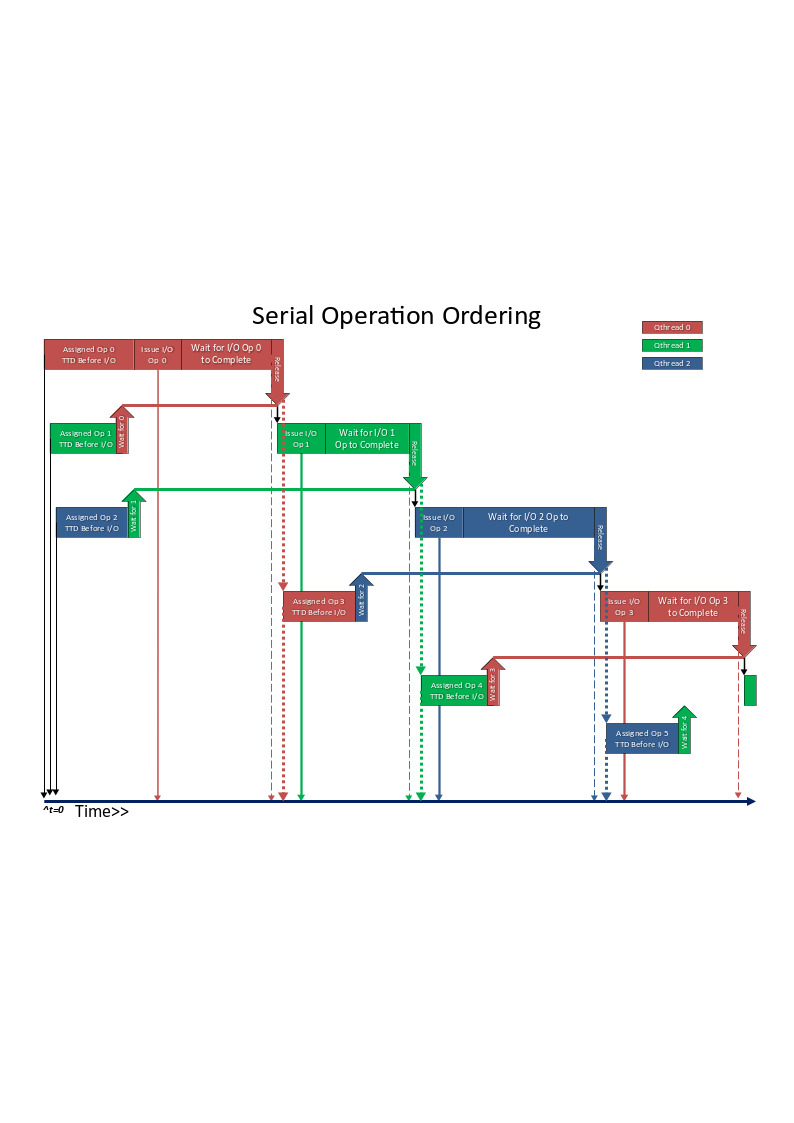
\includegraphics[width=7in,height=5.26736in,alt={Slide1.JPG}]{./images/media/image2.jpg}

\subsubsection{Loose Ordering}\label{loose-ordering}

Loose Ordering is similar to Serial Ordering but is not as strict. In Loose Ordering the QThread responsible for I/O Operation N+1 is supposed to issue its I/O Operation \emph{\ul{after}} I/O Operation N has been \emph{\ul{issued}} but \emph{\ul{before}} I/O Operation N has \emph{\ul{completed}}. The idea is that the storage controller will receive several I/O Operation requests and that after each request finishes, there is another request ready to be executed. There is also the distinct possibility that the subsequent I/O requests have some inherent locality of reference and the storage controller can optimize access to the storage devices based on this locality information.

For example, for purely sequential read operations, if the storage controller sees a consistent, well-ordered set of locations to access it will be able to perform read-ahead operations thereby maximizing the read bandwidth of the underlying storage subsystem. Similarly, for write operations the storage controller could use its write cache more effectively by taking several write operations and coalescing them into a single large write to the storage subsystem.

In practice, Loose Ordering seems to perform better than Serial Ordering for purely sequential read operations because the storage controller always has an I/O Operation to work on.

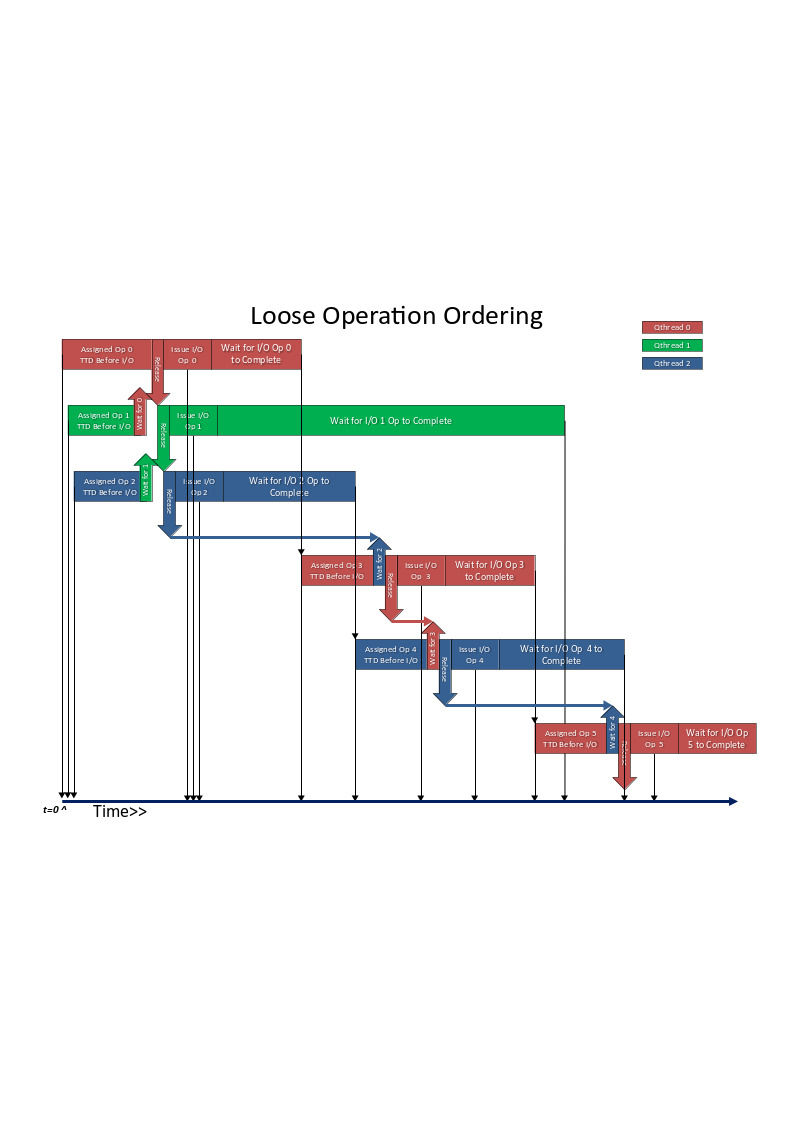
\includegraphics[width=7in,height=5.26736in,alt={Slide2.JPG}]{./images/media/image3.jpg}

\subsubsection{No Ordering}\label{no-ordering}

When No Ordering is used the QThreads will issue their respective I/O Operations without waiting for any prior I/O Operations to complete. The resulting order in which the storage controller sees I/O Operations should be reasonably sequential (in terms of order not necessarily in terms of access locations). However, the order in which the I/O Operations actually get issued depends largely on when the various QThreads are scheduled to run on the system. It has been observed that some QThreads can be ``starved'' for CPU cycles resulting in some I/O Operations experiencing long delays before they are issued and/or completed. This is more an artifact of the Operating System process scheduling algorithms than it is a property of XDD. If I/O Operation ordering is an issue, the Serial and Loose ordering schemes can be used.

\newpage
\section{XDDCP}\label{xddcp}

Xddcp is a shell script located in the ``contrib'' subdirectory of the standard XDD distribution. This shell script is used to copy one or more files from one computer to another over a network. It is intended to be used for very large files, typically in excess of 50 Gigabytes each, over high-speed networks starting at 10Gigabits/sec. Figure XX illustrates the basic operation of XDDCP.

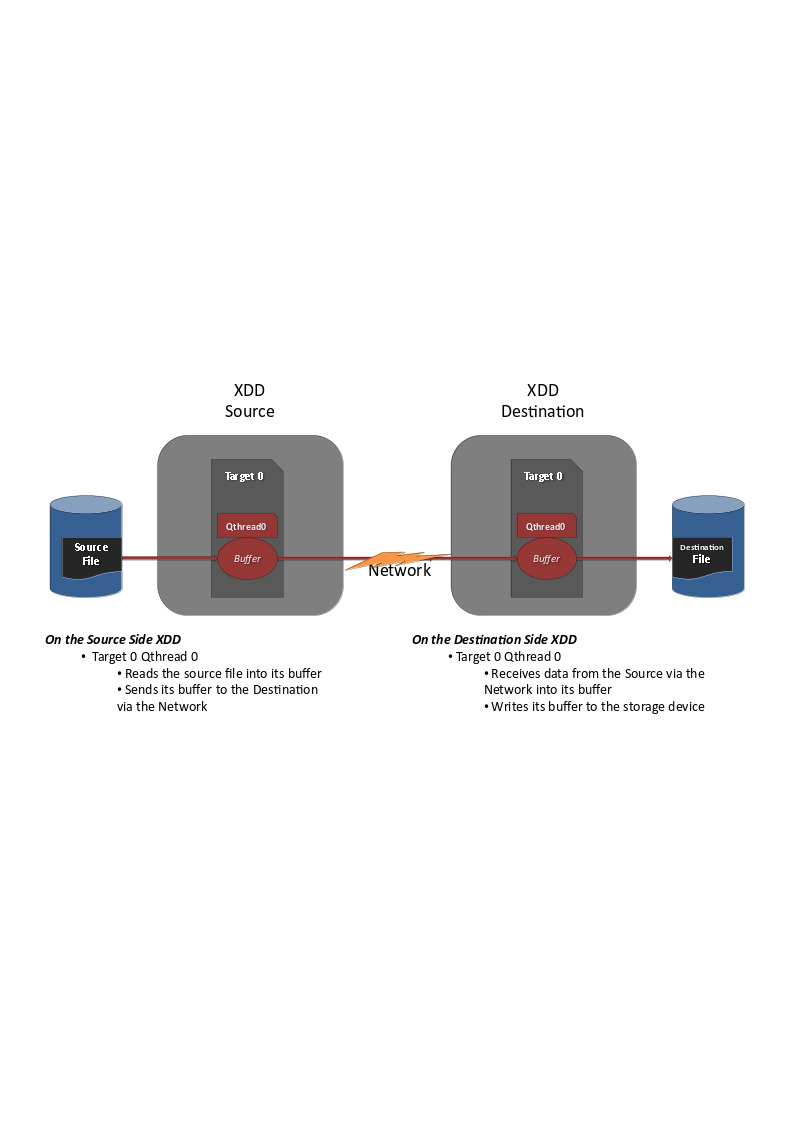
\includegraphics[width=7in,height=3.47917in,alt={Slide1.JPG}]{./images/media/image4.jpg}

Xddcp uses xdd and the End-to-End option to accomplish the data copy operation. It does this by starting an instance of XDD on the ``destination'' computer using ssh and then starting an instance of XDD on the ``source'' computer. The ``source'' side is defined to be where the original file exists. The ``destination'' side is defined to be where the copy of the file will be created.

The destination side is started first and ``listens'' on the specified socket numbers. This version of XDD requires a unique socket number for each ``QThread Pair''. A QThread Pair consists of a source side QThread that sends data to a corresponding destination side QThread through a specific port number.

\subsection{XDDCP Usage}\label{xddcp-usage}

\textbf{xddcp} \emph{{[}OPTIONS{]}} source\emph{\_file destination\_host:destination\_file {[}size{]}}

\begin{quote}
\emph{source\_file} - complete /filepath/name for source file on source host

\emph{destination\_host} - destination host IP or Name over which data is transferred

\emph{destination\_file} - complete /filepath/name for destination file on destination host

\emph{size} - number of bytes to transfer {[}Default: size of source file{]}
\end{quote}

\textbf{\ul{OPTIONS}}

--\textbf{a} -- Specifies that this invocation of xddcp should keep a restart file so that the copy operation can be resumed at a later time if it is interrupted. If this is the resumption of a prior invocation of xddcp then it is used to resume a transfer from the point where the previous invocation was interrupted.

--\textbf{d} -- Use Direct I/O on the destination side of the copy.

--\textbf{s} -- Use direct I/O on the source side of the copy.

--\textbf{f} -- If ports are unavailable on destination, attempt to kill any running XDD's that are running on the destination side and retry starting the destination-side XDD.

--\textbf{F} -- Transfer a list of files named in \emph{source\_file} which is a simple ASCII text file with one file name per line. File names can be either relative or fully qualified path names.

--\textbf{h} -- Print out usage information.

--\textbf{p} \emph{portnum} -- First port to use for transfer {[}Default: 40010{]}. This is also known as the base port.

--\textbf{o} -- Ordered-mode, write data in serial order on the destination side. Normally, no ordering is used on the destination side.

--\textbf{t} \emph{threads} -- Used to specify the number of QThreads to use on the source and destination sides of a copy operation. {[}Default: 8{]}

--\textbf{v} -- Additional information added to the output log files. This will also cause timestamp files to be generated on both the source and destination sides of a copy.

--\textbf{w} -- Same as the --v option but will also generate a binary tim

\textbf{NOTE:} \textquotesingle xdd.Linux\textquotesingle{} must be in your PATH env on both source and destination hosts

\subsection{End-to-End and XDDCP Theory of Operation}\label{end-to-end-and-xddcp-theory-of-operation}

XDDCP uses the End-to-End options to accomplish the task of copying data from one computer to another over a network. The End-to-End operation is accomplished by a ``matched pair'' of XDD instances with one instance running on the ``Source'' computer and the other instance running on the ``Destination'' computer. The ``Source'' computer is defined to be the system that reads in the original file and transmits its contents over a network to the ``Destination'' computer which is defined to be the system that writes the copy of the file to stable storage. Data movement is always from the Source to the Destination.

It is important to note that the Source and Destination instances of XDD must be ``matched'' in the sense that they each have the same queue depth and that they agree on which network addresses and ports to use. For E2E operations the queue depth can either be specified explicitly using the ``-queuedepth'' option or it can be specified implicitly using the ``\textbf{-e2e destination} \emph{hostname:base\_port,number\_of\_ports}'' option. When the queue depth is specified implicitly, it will take precedence over the ``-queuedepth'' option if it is also specified. Furthermore, the queue depth implied on the \textbf{``-e2e destination\ldots''} option is the sum of all ``number\_of\_ports'' specified for a given XDD run.

For example,

The following diagram describes how E2E works with multiple threads:

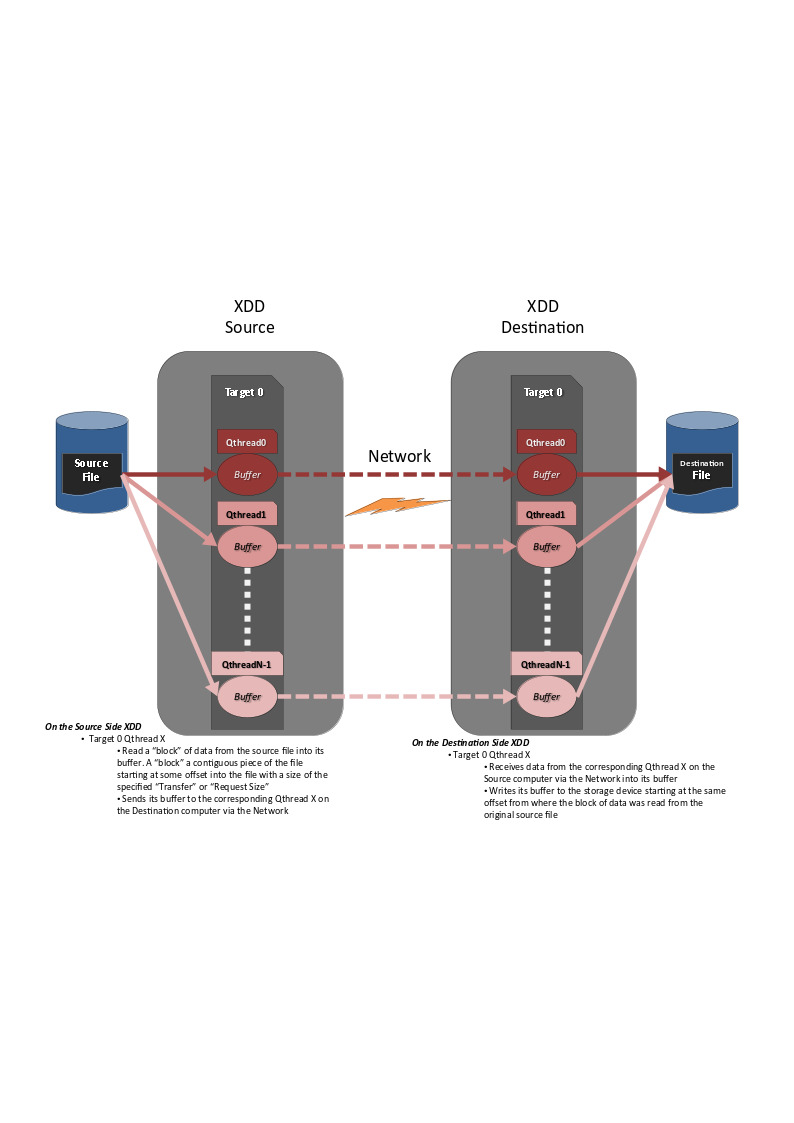
\includegraphics[width=7in,height=5.26736in,alt={Slide2.JPG}]{./images/media/image5.jpg}

XDD can use either buffered I/O or Direct I/O for reading the source file or writing the destination file. Buffered I/O will increase the CPU overhead and possibly result in lower overall bandwidth performance of an E2E operation. Therefore, it is recommended that Direct I/O be used whenever possible. The following diagrams illustrate the basic difference between buffered I/O and Direct I/O as they relate to an E2E operation.

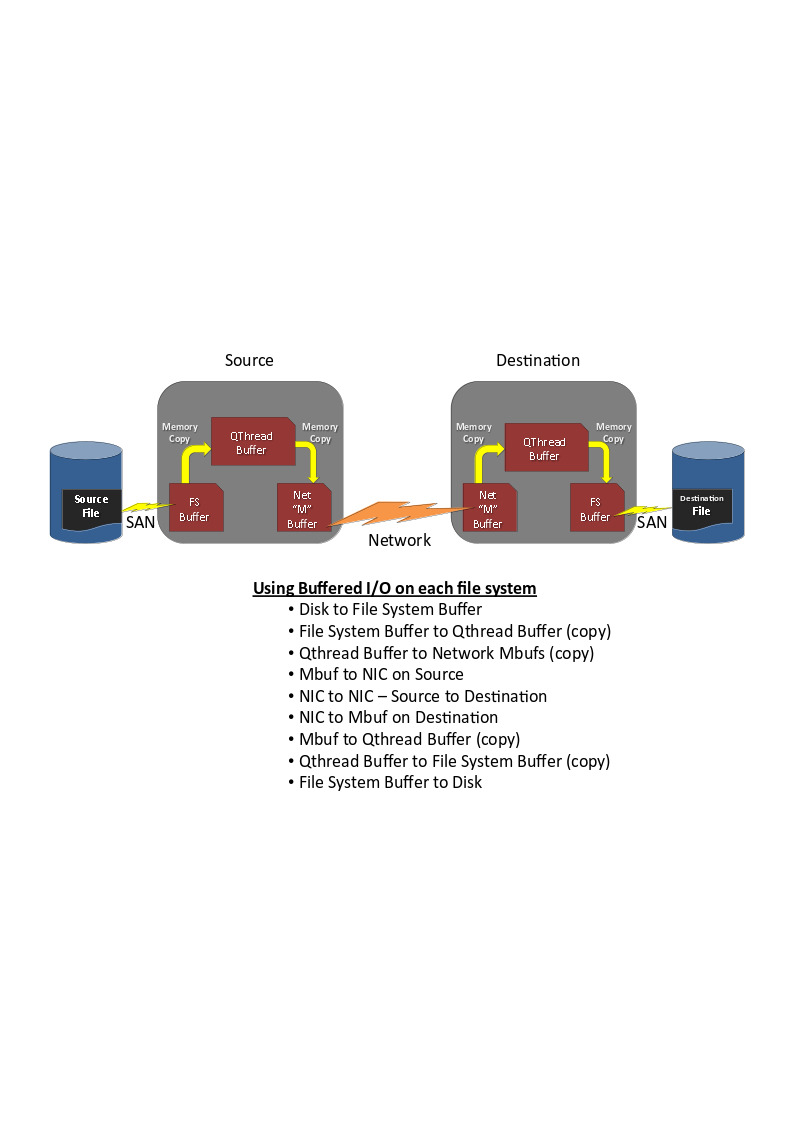
\includegraphics[width=7in,height=4.41667in,alt={Slide3.JPG}]{./images/media/image6.jpg}

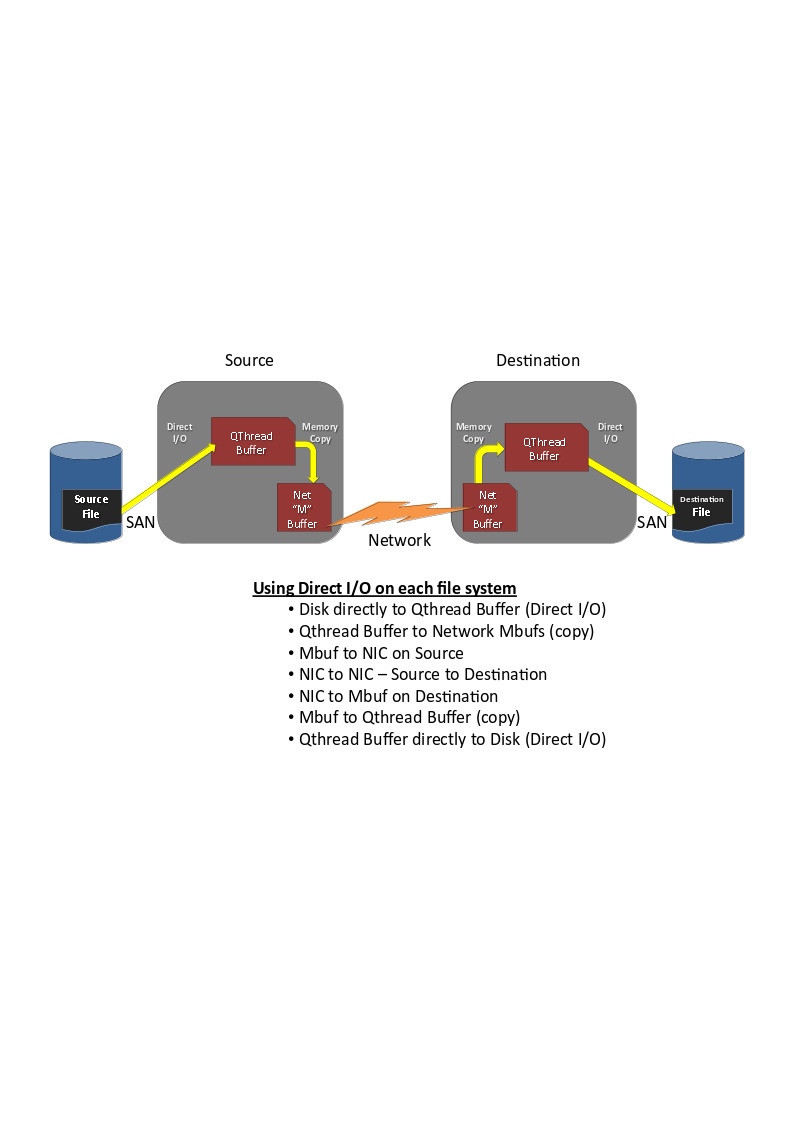
\includegraphics[width=7in,height=4.03125in,alt={Slide4.JPG}]{./images/media/image7.jpg}

\newpage
\section{Runtime Hints}\label{runtime-hints}

\subsection{Windows}\label{windows}

The Windows physical drive is the equivalent of the raw volume in a Unix environment. The physical drive can be specified by using the following XDD command line:

XDD --op read --targets 1 \href{file://///.//PhysicalDrive0}{\textbackslash\textbackslash.\textbackslash\textbackslash PhysicalDrive0} --blocksize 1 --mbytes 1

XDD may complain about an incorrect function but that message can be ignored. It will be fixed in a future release. If a \emph{cygwin} shell window is being used then the syntax must include extra ``\textbackslash'' characters like so:

XDD --op read --targets 1 \textbackslash\textbackslash\textbackslash\textbackslash.\textbackslash\textbackslash\textbackslash\textbackslash PhysicalDrive0 --blocksize 1 --mbytes 1

\subsection{Linux}\label{linux-1}

Raw I/O is only supported using the ``raw'' command to create the ``raw'' device associates and then doing I/O to those devices. The Linux ``raw'' devices are only an approximation of real raw devices on most other Unix systems. It should also be mentioned that transfer sizes larger than about 256Kbytes may not actually be issued to the device but rather be split into multiple requests by the ``raw'' device driver.

\subsection{FreeBSD}\label{freebsd}

\subsection{OSX}\label{osx}

\subsection{Solaris}\label{solaris}

Solaris is no longer supported.

\subsection{IRIX}\label{irix}

IRIX is no longer supported but was reasonably well behaved and had no known idiosyncrasies.

\subsection{\texorpdfstring{AIX }{AIX }}\label{aix-1}

AIX is no longer officially supported.

AIX can use very large page sizes (on the order of 16Mbytes per page) but it is still necessary to ``pin'' all the pages in memory for every I/O operation. For most I/O performance testing this is not a problem unless the number of targets gets large and/or the bandwidth is very high. In this case the page pinning operation takes a significant percentage of the I/O time and can have a negative affect on the results.

To avoid the page pinning penalty, the ``-sharedmemory'' operation can be used to allocate the I/O buffer in a shared memory segment which causes the system to bypass the page pining since shared memory pages are already pinned by default.

\newpage
\section{Output and Reports}\label{output-and-reports}

\subsection{Reporting Options}\label{reporting-options}

The --verbose option will display performance information for each pass within an XDD run along with per-target totals and combined averages. There is also an ``id'' option (--id) that will display a specified string of identification information along with the normal output of the run. If the id string is specified to be ``commandline'' then the entire XDD command line plus all the options will be display. This is useful when running XDD from a shell script to get more qualitative information about the run into the output file.

Since XDD I/O operations can fail due to device failures or option specifications it is possible to generate tremendous numbers of error messages. To avoid filling up output files with too many error messages, the --maxerrors option can be used to limit the number of error messages to display to some small, finite number. Once this number of errors has been reached, I/O operations to that target are halted for that pass.

\subsection{Output Format}\label{output-format}

The ``--outputformat'' option allows the user to specify which variables should be displayed in the output line. For example, given a normal XDD command line with the usual options, it is possible to use the ``-outputformat'' option as follows:

\begin{quote}
XDD \ldots{} -outputformat ``+PASS+TARGET+BYTESREAD+OPS+READBANDWIDTH''
\end{quote}

To produce output that would only contain the pass number, target number, bytes ``read'', operations performed, and achieved ``read'' bandwidth.

The following is a list of defined output format identifier strings that can be used. Each format identifier string must begin with a ``+'' as indicated.

\textbf{+WHAT}

\textbf{+PASS}

\textbf{+TARGET}

\textbf{+QUEUE}

\textbf{+BYTESTRANSFERED}

\textbf{+BYTESXFERED}

\textbf{+BYTESREAD}

\textbf{+BYTESWRITTEN}

\textbf{+OPS}

\textbf{+READOPS}

\textbf{+WRITEOPS}

\textbf{+BANDWIDTH}

\textbf{+READBANDWIDTH}

\textbf{+WRITEBANDWIDTH}

\textbf{+IOPS}

\textbf{+READIOPS}

\textbf{+WRITEIOPS}

\textbf{+LATENCY}

\textbf{+ELAPSEDTIME1STOP}

\textbf{+ELAPSEDTIMEPASS}

\textbf{+OVERHEADTIME}

\textbf{+PATTERNFILLTIME}

\textbf{+BUFFERFLUSHTIME}

\textbf{+CPUTIME}

\textbf{+PERCENTCPUTIME}

\textbf{+PERCENTCPU}

\textbf{+USERTIME}

\textbf{+USER}

\textbf{+USRTIME}

\textbf{+SYSTEMTIME}

\textbf{+SYSTEM}

\textbf{+SYSTIME}

\textbf{+PERCENTUSER}

\textbf{+PERCENTUSERTIME}

\textbf{+PERCENTUSR}

\textbf{+PERCENTSYSTEM}

\textbf{+PERCENTSYSTEMTIME}

\textbf{+PERCENTSYS}

\textbf{+OPTYPE}

\textbf{+XFERSIZEBYTES}

\textbf{+XFERSIZEBLOCKS}

\textbf{+XFERSIZEKBYTES}

\textbf{+XFERSIZEMBYTES}

\textbf{+E2EIOTIME}

\textbf{+E2ESRTIME}

\textbf{+E2EPERCENTSRTIME}

\textbf{+E2ELAGTIME}

\textbf{+E2EPERCENTLAGTIME}

\textbf{+E2EFIRSTREADTIME}

\textbf{+E2ELASTWRITETIME}

\textbf{+DELIM}

** Aside from the obvious ones, the ``+DELIM'' can be used to print a specific delimiter between variables that get displayed. The ``+WHAT'' is used to indicate which output line is being displayed: PASS, QThread Average, Target Average, Combined, \ldots etc. All the others are reasonably self-explanatory

The output of XDD comes in several sections. The first section describes the state of options selected for the run that apply to all the targets being tested. The second section of output describes the options that apply to each of the individual targets. The third section contains information about the system that XDD is being run on. \textbf{The fourth section describes the rate information.}

\textbf{IOIOIOIOIOIOIOIOIOIOI XDD version Linux.7.0.0.rc9.012810.Build.0317 based on Linux.7.0.0.rc9.011810.Build.1412 IOIOIOIOIOIOIOIOIOIOIOI}

\textbf{xdd - I/O Performance Inc., US DoE/DoD Extreme Scale Systems Center \textless ESSC\textgreater{} at Oak Ridge National Labs \textless ORNL\textgreater{} - Copyright 1992-2010}

\textbf{XDD DISCLAIMER:}

\textbf{*** \textgreater\textgreater\textgreater\textgreater{} WARNING \textless\textless\textless\textless{}}

\textbf{*** THIS PROGRAM CAN DESTROY DATA}

\textbf{*** USE AT YOUR OWN RISK}

\textbf{*** IOPERFORMANCE and/or THE AUTHORS ARE NOT LIABLE FOR}

\textbf{*** \textgreater\textgreater\textgreater\textgreater{} ANYTHING BAD \textless\textless\textless\textless{}}

\textbf{**** THAT HAPPENS WHEN YOU RUN THIS PROGRAM}

\textbf{...although we will take credit for anything good that happens}

\textbf{but we are not *liable* for that either.}

\textbf{Starting time for this run, Thu Jan 28 03:22:27 2010}

\textbf{ID for this run, \textquotesingle No ID Specified\textquotesingle{}}

\textbf{Maximum Process Priority, disabled}

\textbf{Passes, 1}

\textbf{Pass Delay in seconds, 0}

\textbf{Maximum Error Threshold, 0}

\textbf{Target Offset, 0}

\textbf{I/O Synchronization, 0}

\textbf{Total run-time limit in seconds, 0}

\textbf{Output file name, test-run.txt}

\textbf{CSV output file name, test-run.csv}

\textbf{Error output file name, stderr}

\textbf{Pass synchronization barriers, enabled}

\textbf{Number of Targets, 1}

\textbf{Number of I/O Threads, 1}

\textbf{Computer Name, pod7.ccs.ornl.gov, User Name, tmruwart}

\textbf{OS release and version, Linux 2.6.18-128.1.6.el5 \#1 SMP Wed Apr 1 06:58:14 EDT 2009}

\textbf{Machine hardware type, x86\_64}

\textbf{Number of processors on this system, 8}

\textbf{Page size in bytes, 4096}

\textbf{Number of physical pages, 8241895}

\textbf{Megabytes of physical memory, 32194}

\textbf{Clock Ticks per second, 100}

\textbf{Seconds before starting, 0}

\textbf{\hfill\break
}

\textbf{Target{[}0{]} Q{[}0{]}, /data/xfs/testfile}

\begin{quote}
\textbf{Target directory, "./"}

\textbf{Process ID, 2523}

\textbf{Thread ID, 2524}

\textbf{Processor, all/any}

\textbf{Read/write ratio, 0.00 READ, 100.00 WRITE}

\textbf{Throttle in MB/sec, 0.00}

\textbf{Per-pass time limit in seconds, 0}

\textbf{Pass seek randomization, disabled}

\textbf{File write synchronization, disabled}

\textbf{Blocksize in bytes, 4194304}

\textbf{Number of Operations, 16, of, 16, target ops for all qthreads}

\textbf{Start offset, 0, blocks, 0, bytes, 0.000 KBytes, 0.000 MBytes, 0.000 GBytes, 0.000000 TBytes}

\textbf{Total data transfer for this target, 65536, blocks, 67108864, bytes, 65536.000 KBytes, 64.000 MBytes, 0.062 GBytes, 0.000061 TBytes}
\end{quote}

\textbf{Total data transfer for this QTHREAD, 65536, blocks, 67108864, bytes, 65536.000 KBytes, 64.000 MBytes, 0.062 GBytes, 0.000061 TBytes}

\textbf{Pass Offset, 0, blocks, 0, bytes, 0.000 KBytes, 0.000 MBytes, 0.000 GBytes, 0.000000 TBytes}

\textbf{Seek range, 1048576, blocks, 1073741824, bytes,1048576.000 KBytes,1024.000 MBytes, 1.000 GBytes, 0.000977 TBytes}

\textbf{Seek pattern, sequential}

\textbf{Flushwrite interval, 0}

\textbf{I/O memory buffer is a normal memory buffer}

\textbf{I/O memory buffer alignment in bytes, 4096}

\textbf{Data pattern in buffer,0x00}

\textbf{Data buffer verification is disabled.}

\textbf{Direct I/O, enabled}

\textbf{Preallocation, 0}

\textbf{Queue Depth, 1}

\textbf{Timestamping, enabled for DETAILED SUMMARY}

\textbf{Timestamp ASCII output file name, test-run.target.0000.qthread.0000.csv}

\textbf{Delete file, disabled}

What Pass Target Queue Bytes\_Xfered Ops Elapsed Bandwidth IOPS Latency Pct\_CPU Op\_Type Xfer\_Size

UNITS\textgreater\textgreater{} Number Number Number Bytes \#ops seconds MBytes/s Ops/s millisec percent text bytes

TARGET\_PASS 1 0 1 67108864 16 1.375 48.820 11.640 85.914 0.727 write 4194304

TARGET\_AVERAGE 1 0 1 67108864 16 1.375 48.820 11.640 85.914 0.727 write 4194304

COMBINED 1 1 1 67108864 16 1.375 48.820 11.640 85.914 0.727 write 4194304

Ending time for this run, Thu Jan 28 03:22:28 2010

The default output of XDD is a line of text with the following format

\textbf{What Pass Target Queue Bytes\_Xfered Ops Elapsed Bandwidth IOPS Latency Pct\_CPU Op\_Type Xfer\_Size}

\textbf{\emph{UNITS\textgreater\textgreater{} Number Number Number Bytes \#ops seconds MBytes/s Ops/s millisec percent text} \emph{bytes}}

The first line indicates the variable being reported, the second line provides the \emph{UNITS} for each variable, and the lines beyond that are the variables themselves.

The fields have the following meanings:

\textbf{WHAT} This is an identifier that explains how the results should be interpreted for the given line. The possible values of ``WHAT'' are:

\begin{itemize}
\item
  TARGET PASS -- displayed only when the --verbose option is specified. Provides the results for a specific target for a particular pass. The target results are a combined average of all the associated qthreads for the target. The ``Q'' result in this case reflects the total number of qthreads operating on behalf of the target.
\item
  QUEUE PASS -- displayed only when the --qthreadinfo option is specified. Provides the results for a specific qthread for a particular pass. The ``Q'' result in this case reflects the specific qthread number relative to zero for this target. For example, if there are 4 qthreads (i.e. --queuedepth 4) then the Q values will range from 0 to 3.
\item
  TARGET AVERAGE -- displayed only when the --verbose option is specified. Provides the results for a specific target averaged over all passes in the run.
\item
  COMBINED -- Provides the combined results over all targets and qthreads for all passes in a run.
\end{itemize}

\textbf{PASS} is the target pass number of the specific result. Pass numbers start at 1.

\textbf{Target} is the target number, relative to 0 (zero). A list of the targets and the associated numbers precedes this line of output.

\textbf{Queue} -- see above.

\textbf{Bytes\_Xfered} Is the total number of bytes that were transferred during the XDD run for this target.

\textbf{Ops} is the total number of read or write operations performed on this target.

\textbf{Elapsed} is the number of seconds that elapsed for the current pass in a multi-pass run for the target or qthread being reported.

\textbf{Bandwidth} is the average I/O rate in Mega Bytes per Second where 1 MByte/sec equally 10\textsuperscript{6} bytes per second.

\textbf{IOPS} is the Average number of I/O operations per second for this pass in a multi-pas run.

\textbf{Latency} is the Average time it takes to perform each operation.

\textbf{Pct\_CPU} is the percentage of the CPU that was used by all the qthreads on behalf of this target. This includes system and user time.

\textbf{Op\_type} is either read, write, or mixed.

\textbf{Xfer\_Size} is the *average* transfer size represented as block-size that was used for that target or qthread. Generally this is a constant value for any particular test run.

If the \textbf{--verbose} option is specified then each line has a pass number associated with it and the final output lines report overall averaged values for the Average Rate and Elapsed time. For a Multi-Target run, the sum total of all the targets is presented as the \textbf{Combined} average. For example, if \emph{two} targets are being tested and \emph{each} target performs at an average of 75MB/sec, the Combined average is 150 MB/sec.

\subsection{}\label{section}

\subsection{What the numbers really mean}\label{what-the-numbers-really-mean}

There are several performance values reported. These include the per-pass target results, the individual queue results, the target averages over all passes, and the combined average of all targets over all passes.

\newpage
\section{Performance Tuning Hints}\label{performance-tuning-hints}

This section describes various hints about performance tuning.

\subsection{\texorpdfstring{Caches and write performance }{Caches and write performance }}\label{caches-and-write-performance}

When writing to a storage device whether it is a single disk drive or a disk array it is important to know the status of the caches on each of the devices that have cache. For maximum performance for write operations, it is necessary to enable the write caches on a disk array controller as well as the write caches on the disk drives themselves.

\subsection{Fibre Channel Frame Sizes}\label{fibre-channel-frame-sizes}

Fibre Channel host bus adapters (HBA), switches, and target devices all have frame sizes defined and negotiated when any two FC devices are connected together. For maximum bandwidth performance it is important to make certain that the FC frame size is set to 2048-bytes. For maximum transaction performance for small transaction sizes (i.e. around 512 bytes per transaction) a smaller frame size of 512 or 1024 bytes can be used.

\newpage
\section{Examples}\label{examples}

The following is a list of examples on how to run XDD.

\subsection{Example 1 -- Basic XDD command line}\label{example-1-basic-xdd-command-line}

\begin{quote}
XDD --op \textbf{read} --targets \textbf{1} \textbf{/dev/rdsk/dsk10d2s0} --blocksize \textbf{128}

-mbytes \textbf{64} --passes \textbf{3} --verbose
\end{quote}

This is a very basic test that will \textbf{read} sequentially from target device \textbf{/dev/rdsk/dks10d2s0} starting at block 0 using a fixed block size of \textbf{128} bytes until it has read \textbf{64} MegaBytes (64 *1024*1024 bytes). It will do this \textbf{3} times and display performance information for each pass. Please note that all these options need to be on a single command line unless they are in the setup file where they can be on separate lines.

\subsection{Example 2 -- Specifying multiple targets and timelimit}\label{example-2-specifying-multiple-targets-and-timelimit}

\begin{quote}
XDD --op \textbf{write} --targets \textbf{2 /raid/BIGFILE1 /raid/BIGFILE2}

-blocksize \textbf{512} -mbytes \textbf{64} --verbose

--passes \textbf{3} -timelimit \textbf{10}
\end{quote}

This test will \textbf{write} sequentially from \textbf{2} target files \textbf{/raid/BIGFILE1} and \textbf{/raid/BIGFILE2} starting at the beginning of each file using a fixed block size of \textbf{512} bytes until it has read \textbf{64} MegaBytes (64 * 1024*1024 bytes) \emph{-- or --} until it has reached a time limit of \textbf{10} seconds at which time it will end the current pass and proceed to the next pass. It will do this \textbf{3} times and display performance information for each pass. The \emph{combined} performance of both devices is calculated and displayed at the end of the run.

\subsection{Example 3 -- Time Stamping and Setup File}\label{example-3-time-stamping-and-setup-file}

\begin{quote}
XDD --op \textbf{write} --targets \textbf{2 /dev/rdsk/dks10d2s0 /dev/rdsk/dks10d2s0}

-setup \textbf{XDD.setup} --ts \textbf{detailed} --ts output \textbf{ts.write}
\end{quote}

This test that will \textbf{read} sequentially from \textbf{2} targets that are actually a single device: \textbf{/dev/rdsk/dks10d2s0.} The transfer size of \textbf{2048} bytes per block, read limit of \textbf{4096} MegaBytes (4096 * 1024*1024 bytes), the time limit of \textbf{10} seconds for each pass, verbose output, and pass count of \textbf{3} are all specified in the \textbf{XDD.setup} file which looks like so:

\begin{quote}
-blocksize \textbf{2048}

-mbytes \textbf{4096}

--verbose

--passes \textbf{3} -timelimit \textbf{10}
\end{quote}

The time stamp option is also used in this example to dump an ASCII output file called \textbf{ts.write.} It should be noted that these time stamp file names are appended with a \textbf{t\#} where \textbf{\#} is the number of the target that belongs to the particular time stamp file. In this example, since there are two targets, the time stamp files will be \textbf{ts.write.t0} and \textbf{ts.write.t1.}

\subsection{\texorpdfstring{Example 4 -- Random Seeks }{Example 4 -- Random Seeks }}\label{example-4-random-seeks}

\begin{quote}
XDD --op \textbf{read} --targets \textbf{1} \textbf{/dev/rdsk/dsk10d2s0} --blocksize \textbf{1024}

-mbytes \textbf{16} --passes \textbf{3} --verbose

--seek random --seek range \textbf{4000000}
\end{quote}

This is a very basic \emph{random I/O} test that will \textbf{read} from target device \textbf{/dev/rdsk/dks10d2s0} starting at some random location in \textbf{1024-byte} blocks until it has read \textbf{16} MegaBytes (16 * 1024*1024 bytes). It will do this \textbf{3} times and display performance information for each pass. The number of requests that need to be generated to read 16 MegaBytes in 1024 byte blocks is 16,384. Since this is a purely random I/O pattern, these 16,384 requests are distributed over a range of 4,000,000 blocks (again 1024 bytes per block). This is useful in constraining the area over which the random locations are chosen from. The same seek locations are used for each pass in order to generate reproducible results. In fact, upon each invocation of XDD using the same parameters, the same random locations are generated each time. This allows the user to change the disk or starting offset or some such thing and observe the effects. The random locations may be changed from pass to pass within an XDD run by using the "-\textbf{randomize}" option in which case a new set of locations is generated for each pass. Furthermore, the random locations may be changed from run to run using the \textbf{--seek seed} option to specify a different random number generation seed value for each invocation of XDD.

\subsection{Example 5 -- End to End operation}\label{example-5-end-to-end-operation}

Perform an end to end operation between two hosts, hostA and hostB, where hostA is the \emph{source} and hostB is the \emph{destination}.

Start the instance of XDD on hostB, the \emph{destination} side \ul{first}. This is required because if the \emph{destination} side is not running when the \emph{source} side starts, the \emph{source} side will terminate early because it will not be able to connect to the instance of XDD on the \emph{destination} side.

Hence, on the \emph{destination} side:

\begin{quote}
XDD --op \textbf{write} --targets \textbf{1} \textbf{/tmp/foo2} --blocksize \textbf{4096} -mbytes \textbf{3000} --verbose \textbackslash{}

--e2e \textbf{isdestination} --e2e \textbf{destination} \textbf{192.168.17.10} --e2e \textbf{port 2010}
\end{quote}

Once this is running it will wait for a connection from the \emph{source} side before writing data to the \emph{destination} target file \textbf{/tmp/foo2.}

On the \emph{source} side:

\begin{quote}
XDD --op \textbf{read} --targets \textbf{1} \textbf{/tmp/foo1} --blocksize \textbf{4096} -mbytes \textbf{3000} --verbose \textbackslash{}

--e2e \textbf{issource} --e2e \textbf{destination} \textbf{192.168.17.10} --e2e \textbf{port 2010}
\end{quote}

Once the \emph{source} side starts, it will open a socket to the \emph{destination} host and start reading the \emph{source} file \textbf{/tmp/foo1} and sending it over the socket to the \emph{destination} side.

Once the target file on the \emph{source} side has been read and transferred, assuming no additional passes are requested, then the \emph{source} side will terminate followed by the \emph{destination} side. Each will display the usual results with an additional value at the end of each output line. This value will be a number between 0 and 100 and represents the percentage of total time that was spent by XDD transferring data over the network.

It is important to follow these basic rules when running an e2e operation:

\begin{itemize}
\item
  The source and destination XDD command lines must contain either --e2e issource or --e2e isdestination respectively in order to properly identify their respective roles
\item
  The ``operation'' or --op for the \emph{source} must be ``read''
\item
  The ``operation'' or --op for the \emph{destination} must be ``write''
\item
  The number of megabytes to read from the \emph{source} target should be equal to the number of megabytes written to the \emph{destination} target
\item
  The queue depth (i.e. --queuedepth option) must be the same on both the \emph{source} and \emph{destination} sides for a given target
\item
  The \emph{destination} host name/address must be specified on both \emph{source} and \emph{destination} \emph{XDD} command lines and must be the same
\end{itemize}

\subsection{E2E Example with multiple Network Interfaces}\label{e2e-example-with-multiple-network-interfaces}

\textbf{\ul{On the~Source~Side:}}

xdd .....~

~~ -targets 1 null ~ ~ ~ ~ ~ ~ ~ ~ \# Will read or write using the XDD null device

\textbf{~~ -op ~read ~ ~ ~ ~ ~ ~ ~ ~ ~\# Read from the source file/device}

~~~\textbf{-e2e~issource ~ ~ ~ ~ ~ ~ ~ ~ \# Specifies that this is the Source side}

~~~\textbf{-e2e~destination~\href{http://192.168.1.5:40010/}{192.168.1.5:40010},4 \# Specifies the first~destination~side address}

\textbf{\# to use plus the base port and number of ports}

\textbf{~~ -e2e~destination~\href{http://192.168.2.5:40010/}{192.168.2.5:40010},4 ~ \# Specifies the second~destination side address}

\textbf{\# to use plus the base port and number of ports}

\textbf{~~ -e2e~destination~\href{http://192.168.3.5:40010/}{192.168.3.5:40010},4 ~ \# Specifies the third~destination~side address}

\textbf{\# to use plus the base port and number of ports}

\textbf{~~ -e2e~destination~\href{http://192.168.4.5:40010/}{192.168.4.5:40010},4 ~ \# Specifies the fourth~destination side address}

\textbf{\# to use plus the base port and number of ports}

\textbf{\ul{On the~Destination~Side:}}

~

~~ xdd ...

\textbf{~~ -op ~write ~ ~ ~ ~ ~ ~ ~ ~ ~ ~ ~ ~ \# Write to the~destination~file}

\textbf{~~~-e2e~isdestination \textbackslash{} ~ ~ ~ ~ ~ ~ ~ \# Specifies that this is the Destination side}

~~~\textbf{-e2e~destination~\href{http://192.168.1.5:40010/}{192.168.1.5:40010},4 \# Specifies the first~destination~side address}

\textbf{\# to use plus the base port and number of ports}

\textbf{~~ -e2e~destination~\href{http://192.168.2.5:40010/}{192.168.2.5:40010},4 ~ \# Specifies the second~destination side address}

\textbf{\# to use plus the base port and number of ports}

\textbf{~~ -e2e~destination~\href{http://192.168.3.5:40010/}{192.168.3.5:40010},4 ~ \# Specifies the third~destination~side address}

\textbf{\# to use plus the base port and number of ports}

\textbf{~~ -e2e~destination~\href{http://192.168.4.5:40010/}{192.168.4.5:40010},4 ~ \# Specifies the fourth~destination side address}

\textbf{\# to use plus the base port and number of ports}

plus all the other options\ldots{}

\subsection{Example Time Stamp Output}\label{example-time-stamp-output}

Target and Qthread number for this report, 0, 0

IOIOIOIOIOIOIOIOIOIOI XDD version Linux.7.0.0.rc9.012810.Build.0317 based on Linux.7.0.0.rc9.011810.Build.1412 IOIOIOIOIOIOIOIOIOIOIOI

xdd - I/O Performance Inc., US DoE/DoD Extreme Scale Systems Center \textless ESSC\textgreater{} at Oak Ridge National Labs \textless ORNL\textgreater{} - Copyright 1992-2010

XDD DISCLAIMER:

*** \textgreater\textgreater\textgreater\textgreater{} WARNING \textless\textless\textless\textless{}

*** THIS PROGRAM CAN DESTROY DATA

*** USE AT YOUR OWN RISK

*** IOPERFORMANCE and/or THE AUTHORS ARE NOT LIABLE FOR

*** \textgreater\textgreater\textgreater\textgreater{} ANYTHING BAD \textless\textless\textless\textless{}

**** THAT HAPPENS WHEN YOU RUN THIS PROGRAM

...although we will take credit for anything good that happens

but we are not *liable* for that either.

Starting time for this run, Thu Jan 28 03:22:28 2010

ID for this run, \textquotesingle No ID Specified\textquotesingle{}

Maximum Process Priority, disabled

Passes, 1

Pass Delay in seconds, 0

Maximum Error Threshold, 16

Target Offset, 0

I/O Synchronization, 0

Total run-time limit in seconds, 0

Output file name, test-run.txt

CSV output file name, test-run.csv

Error output file name, stderr

Pass synchronization barriers, enabled

Number of Targets, 1

Number of I/O Threads, 1

Computer Name, pod7.ccs.ornl.gov, User Name, tmruwart

OS release and version, Linux 2.6.18-128.1.6.el5 \#1 SMP Wed Apr 1 06:58:14 EDT 2009

Machine hardware type, x86\_64

Number of processors on this system, 8

Page size in bytes, 4096

Number of physical pages, 8241895

Megabytes of physical memory, 32194

Clock Ticks per second, 100

Seconds before starting, 0

Target{[}0{]} Q{[}0{]}, /data/xfs/testfile

Target directory, "./"

Process ID, 2523

Thread ID, 2524

Processor, all/any

Read/write ratio, 0.00 READ, 100.00 WRITE

Throttle in MB/sec, 0.00

Per-pass time limit in seconds, 0

Pass seek randomization, disabled

File write synchronization, disabled

Blocksize in bytes, 4194304

Number of Operations, 16, of, 16, target ops for all qthreads

Start offset, 0, blocks, 0, bytes, 0.000 KBytes, 0.000 MBytes, 0.000 GBytes, 0.000000 TBytes

Total data transfer for this target, 65536, blocks, 67108864, bytes, 65536.000 KBytes, 64.000 MBytes, 0.062 GBytes, 0.000061 TBytes

Total data transfer for this QTHREAD, 65536,blocks, 67108864, bytes, 65536.000 KBytes, 64.000 MBytes, 0.062 GBytes, 0.000061 TBytes

Pass Offset, 0, blocks, 0, bytes, 0.000 KBytes, 0.000 MBytes, 0.000 GBytes, 0.000000 TBytes

Seek range, 1048576, blocks, 1073741824, bytes, 1048576.000 KBytes, 1024.000 MBytes, 1.000 GBytes, 0.000977 TBytes

Seek pattern, sequential

Flushwrite interval, 0

I/O memory buffer is a normal memory buffer

I/O memory buffer alignment in bytes, 4096

Data pattern in buffer,0x00

Data buffer verification is disabled.

Direct I/O, enabled

Preallocation, 0

Queue Depth, 1

Timestamping, enabled for DETAILED SUMMARY

Timestamp ASCII output file name, test-run.target.0000.qthread.0000.csv

Delete file, disabled

Start of DETAILED Time Stamp Report, Number of entries, 16, Picoseconds per clock tick, 1000000, delta, 0

Target, RWV Op, Pass, OP Number, Block Location, Distance, StartTS, EndTS, IO\_Time\_ms, Relative\_ms, Delta\_us, Loop\_ms, Inst MB/sec

0,w,1,0,0,0,10288350303715490112,10288350437959490112, 134.24400, 0.00000, 0.00000, 0.00000, 31.244

0,w,1,1,4096,0,10288350437966490112,10288350478994490112, 41.02800, 134.25100, 7.00000, 41.03500, 102.230

0,w,1,2,8192,0,10288350478997490112,10288350533440490112, 54.44300, 175.28200, 3.00000, 54.44600, 77.040

0,w,1,3,12288,0,10288350533446490112,10288350736743490112, 203.29700, 229.73100, 6.00000, 203.30300, 20.631

0,w,1,4,16384,0,10288350736750490112,10288350789934490112, 53.18400, 433.03500, 7.00000, 53.19100, 78.864

0,w,1,5,20480,0,10288350789937490112,10288350839706490112, 49.76900, 486.22200, 3.00000, 49.77200, 84.275

0,w,1,6,24576,0,10288350839708490112,10288350973728490112, 134.02000, 535.99300, 2.00000, 134.02200, 31.296

0,w,1,7,28672,0,10288350973733490112,10288351026693490112, 52.96000, 670.01800, 5.00000, 52.96500, 79.198

0,w,1,8,32768,0,10288351026697490112,10288351109349490112, 82.65200, 722.98200, 4.00000, 82.65600, 50.747

0,w,1,9,36864,0,10288351109354490112,10288351173507490112, 64.15300, 805.63900, 5.00000, 64.15800, 65.380

0,w,1,10,40960,0,10288351173509490112,10288351250697490112, 77.18800, 869.79400, 2.00000, 77.19000, 54.339

0,w,1,11,45056,0,10288351250703490112,10288351290625490112, 39.92200, 946.98800, 6.00000, 39.92800, 105.062

0,w,1,12,49152,0,10288351290627490112,10288351353374490112, 62.74700, 986.91200, 2.00000, 62.74900, 66.845

0,w,1,13,53248,0,10288351353380490112,10288351431280490112, 77.90000, 1049.66500, 6.00000, 77.90600, 53.842

0,w,1,14,57344,0,10288351431284490112,10288351621563490112, 190.27900, 1127.56900, 4.00000, 190.28300, 22.043

0,w,1,15,61440,0,10288351621569490112,10288351678337490112, 56.76800, 1317.85400, 6.00000, 56.77400, 73.885

End of DETAILED Time Stamp Report

Start of SUMMARY Time Stamp Report

Average seek distance in 1024 byte blocks, 0

Range: Longest seek distance in blocks, 0, shortest seek distance in blocks, 0

Average I/O time in milliseconds, 77.51937, average dead time in microseconds, 4.53333

I/O Time Range: Longest I/O time in milliseconds, 203.29700, shortest I/O time in milliseconds, 39.92200

Dead Time Range: Longest dead time in microseconds, 7.00000, shortest dead time in microseconds, 2.00000

End of SUMMARY Time Stamp Report

\newpage
\section{\texorpdfstring{\hfill\break
Under the Hood}{ Under the Hood}}\label{under-the-hood}

This section is a look at XDD program organization and data structures. This section is primarily here for the author's benefit because his brain is getting old and forgetful.

Starting with XDD6.3 the source code files have been separated out into several categories of source files. The process of moving functions around within the files is mostly complete but further changes may be made in future releases. The rationale behind this change is that some of the source files were getting too large.

\subsection{XDD general operation}\label{xdd-general-operation}

XDD is a command-line driven program. The first thing it does upon invoking it is to parse the command line. If the command line contains the ``-setup'' option, it will parse the command line options from left to right up to the --setup option. It will then parse the setup file options followed by parsing the remaining command line options.

After the all the requested options have been set, the main XDD program will start all the appropriate threads one at a time. Each thread will go through it initialization phase which includes the following:

\begin{itemize}
\item
  Open the target and prepare it for access
\item
  Generate the list of locations to access and the associated access pattern and operations
\item
  Allocate I/O buffer
\item
  Perform timestamp setup if necessary
\item
  Display target-specific information as requested
\end{itemize}

After the thread has completed its setup process, it will enter a serialization barrier that will release the main XDD parent thread which will in turn start the next thread. The target thread that has just completed initialization will enter the main barrier waiting for all the other target threads to complete initialization. Once all the threads have been started, the last thread to start will enter the starting barrier and cause all the threads to be released and the fun begins.

All the threads will do their respective I/O operations for a single pass and then enter the pass barrier. The pass barrier causes threads to wait until all threads have completed a pass before starting the next pass. If this is the last pass, then upon being released from this barrier, all the threads will perform any clean-up operations and exit.

Another function of the pass barrier is to hold all the threads dormant whilst thread 0 gathers all the results information from each of the threads and generates the appropriate intermediate results and displays them if requested. This is also the case when all threads have completed all passes and thread 0 needs to process summary information as well.

\subsection{The XDD buffer memory layout}\label{the-xdd-buffer-memory-layout}

XDD uses several buffers during a normal run. All buffers are page aligned. These buffers include:

\begin{itemize}
\item
  The Read/Write I/O buffer. This buffer is simply the size of a single I/O request and there is one of these buffers per target being tested. This buffer is normally allocated from user space memory but if the ``-sharedmemory'' option is specified the buffer will be allocated from a shared memory segment. The use of a shared memory segment can have a significant impact on bandwidth performance in some cases.
\item
  Access location / operation buffer (aka seeklist). This buffer is variable in size and depends on the number of I/O operations that need to be performed. There is one access location/operation buffer for each target being tested. This buffer contains the following information:

  \begin{itemize}
  \item
    The block location to access
  \item
    The operation to be performed (read or write)
  \item
    The amount of data to transfer for that operation
  \item
    The time to issue the I/O request
  \end{itemize}
\item
  Time stamp buffer if time stamping is enabled. This buffer can get very large because there is one time stamp entry for every I/O operation to be performed for the entire XDD run (which includes all passes). For example, if there are three targets and each target will perform 8192 operations per pass and there are 4 passes, then there will be three time stamp buffers (one for each target) with 32768 entries in each buffer (4 passes times 8192 entries per pass). Each time stamp entry contains the following information:

  \begin{itemize}
  \item
    Start time stamp (64-bit)
  \item
    End time stamp (64-bit)
  \item
    Operation (read or write)
  \item
    Amount of data transferred
  \item
    Pass number
  \item
    Operation number
  \end{itemize}
\item
  Per Thread Data Structure (ptds). This data structure contains all the information related to a single target during an XDD run. This is explained in more detail in the section on the \emph{XDD thread structure}.
\end{itemize}

\subsection{The XDD thread structure}\label{the-xdd-thread-structure}

XDD uses POSIX threads for all processes that it controls. There are one or more threads per target. Each target will have a primary thread and potentially some number of Q threads. The Q threads are used to perform parallel, asynchronous I/O on a particular target. The concept of Q threads is essentially ``aio'' but since ``aio'' is different from system to system, it was easier to simply implement one within XDD.

Each thread (primary or Q thread) has a PTDS (\ul{p}er \ul{t}hread \ul{d}ata \ul{s}tructure) data structure associated with it. The PTDS contains all the information related to a thread running at any given time. This structure is passed to the various routines within XDD. The PTDS's are allocated on an as-needed basis. The layout of the PTDS structures is shown in Figure 1.

The Per Target Data Structure (PTDS) layout including the QThreads.

In the above diagram there are N targets each with some number of QThreads. The number of QThreads is equal to the Queue Depth specified for each target (using the --queuedepth option). The number of QThreads can be different for each target as is shown in this diagram but in practice the number of QThreads is the same for all targets during a run. The primary PTDS for each target is, in fact, QThread 0. If there is more than one QThread for a target, the subsequent QThreads are chained together as shown in the diagram. The last QThread in the chain is identified by the fact that its ``next QThread'' point is null.

\subsection{XDD barriers}\label{xdd-barriers}

XDD uses a number of synchronization barriers in order to provide precise control and certain functionality such as lock-stepping. The primary barriers cause all the threads to begin execution at precisely the same time for each pass of a run. The barriers are implemented using mutexes and semaphores. The amount of time required to process a semaphore request is significantly less than the time scales of an I/O operation and has no measurable effect on the results.

\newpage
\section{The GNU Public License}\label{the-gnu-public-license}

Version 2, June 1991

Copyright (C) 1989, 1991 Free Software Foundation, Inc.

59 Temple Place - Suite 330, Boston, MA 02111-1307, USA

Everyone is permitted to copy and distribute verbatim copies of this license document, but changing it is not allowed.

\subsection{\texorpdfstring{\href{http://www.gnu.org/licenses/gpl.html\#TOC2}{\protect\hypertarget{_Toc290917472}{}{}Preamble}}{Preamble}}\label{preamble}

The licenses for most software are designed to take away your freedom to share and change it. By contrast, the GNU General Public License is intended to guarantee your freedom to share and change free software-\/-to make sure the software is free for all its users. This General Public License applies to most of the Free Software Foundation\textquotesingle s software and to any other program whose authors commit to using it. (Some other Free Software Foundation software is covered by the GNU Library General Public License instead.) You can apply it to your programs, too.

When we speak of free software, we are referring to freedom, not price. Our General Public Licenses are designed to make sure that you have the freedom to distribute copies of free software (and charge for this service if you wish), that you receive source code or can get it if you want it, that you can change the software or use pieces of it in new free programs; and that you know you can do these things.

To protect your rights, we need to make restrictions that forbid anyone to deny you these rights or to ask you to surrender the rights. These restrictions translate to certain responsibilities for you if you distribute copies of the software, or if you modify it.

For example, if you distribute copies of such a program, whether gratis or for a fee, you must give the recipients all the rights that you have. You must make sure that they, too, receive or can get the source code. And you must show them these terms so they know their rights.

We protect your rights with two steps: (1) copyright the software, and (2) offer you this license which gives you legal permission to copy, distribute and/or modify the software.

Also, for each author\textquotesingle s protection and ours, we want to make certain that everyone understands that there is no warranty for this free software. If the software is modified by someone else and passed on, we want its recipients to know that what they have is not the original, so that any problems introduced by others will not reflect on the original authors\textquotesingle{} reputations.

Finally, any free program is threatened constantly by software patents. We wish to avoid the danger that redistributors of a free program will individually obtain patent licenses, in effect making the program proprietary. To prevent this, we have made it clear that any patent must be licensed for everyone\textquotesingle s free use or not licensed at all.

The precise terms and conditions for copying, distribution and modification follow.

\subsection{\texorpdfstring{\href{http://www.gnu.org/licenses/gpl.html\#TOC3}{\protect\hypertarget{_Toc290917473}{}{}TERMS AND CONDITIONS FOR COPYING, DISTRIBUTION AND MODIFICATION}}{TERMS AND CONDITIONS FOR COPYING, DISTRIBUTION AND MODIFICATION}}\label{terms-and-conditions-for-copying-distribution-and-modification}

\textbf{0.} This License applies to any program or other work which contains a notice placed by the copyright holder saying it may be distributed under the terms of this General Public License. The "Program", below, refers to any such program or work, and a "work based on the Program" means either the Program or any derivative work under copyright law: that is to say, a work containing the Program or a portion of it, either verbatim or with modifications and/or translated into another language. (Hereinafter, translation is included without limitation in the term "modification".) Each licensee is addressed as "you".

Activities other than copying, distribution and modification are not covered by this License; they are outside its scope. The act of running the Program is not restricted, and the output from the Program is covered only if its contents constitute a work based on the Program (independent of having been made by running the Program). Whether that is true depends on what the Program does.

\textbf{1.} You may copy and distribute verbatim copies of the Program\textquotesingle s source code as you receive it, in any medium, provided that you conspicuously and appropriately publish on each copy an appropriate copyright notice and disclaimer of warranty; keep intact all the notices that refer to this License and to the absence of any warranty; and give any other recipients of the Program a copy of this License along with the Program.

You may charge a fee for the physical act of transferring a copy, and you may at your option offer warranty protection in exchange for a fee.

\textbf{2.} You may modify your copy or copies of the Program or any portion of it, thus forming a work based on the Program, and copy and distribute such modifications or work under the terms of Section 1 above, provided that you also meet all of these conditions:

\textbf{a)} You must cause the modified files to carry prominent notices stating that you changed the files and the date of any change.

\textbf{b)} You must cause any work that you distribute or publish, that in whole or in part contains or is derived from the Program or any part thereof, to be licensed as a whole at no charge to all third parties under the terms of this License.

\textbf{c)} If the modified program normally reads commands interactively when run, you must cause it, when started running for such interactive use in the most ordinary way, to print or display an announcement including an appropriate copyright notice and a notice that there is no warranty (or else, saying that you provide a warranty) and that users may redistribute the program under these conditions, and telling the user how to view a copy of this License. (Exception: if the Program itself is interactive but does not normally print such an announcement, your work based on the Program is not required to print an announcement.)

These requirements apply to the modified work as a whole. If identifiable sections of that work are not derived from the Program, and can be reasonably considered independent and separate works in themselves, then this License, and its terms, do not apply to those sections when you distribute them as separate works. But when you distribute the same sections as part of a whole which is a work based on the Program, the distribution of the whole must be on the terms of this License, whose permissions for other licensees extend to the entire whole, and thus to each and every part regardless of who wrote it.

Thus, it is not the intent of this section to claim rights or contest your rights to work written entirely by you; rather, the intent is to exercise the right to control the distribution of derivative or collective works based on the Program.

In addition, mere aggregation of another work not based on the Program with the Program (or with a work based on the Program) on a volume of a storage or distribution medium does not bring the other work under the scope of this License.

\textbf{3.} You may copy and distribute the Program (or a work based on it, under Section 2) in object code or executable form under the terms of Sections 1 and 2 above provided that you also do one of the following:

\begin{itemize}
\item
  \textbf{a)} Accompany it with the complete corresponding machine-readable source code, which must be distributed under the terms of Sections 1 and 2 above on a medium customarily used for software interchange; or,
\item
  \textbf{b)} Accompany it with a written offer, valid for at least three years, to give any third party, for a charge no more than your cost of physically performing source distribution, a complete machine-readable copy of the corresponding source code, to be distributed under the terms of Sections 1 and 2 above on a medium customarily used for software interchange; or,
\item
  \textbf{c)} Accompany it with the information you received as to the offer to distribute corresponding source code. (This alternative is allowed only for noncommercial distribution and only if you received the program in object code or executable form with such an offer, in accord with Subsection b above.)
\end{itemize}

The source code for a work means the preferred form of the work for making modifications to it. For an executable work, complete source code means all the source code for all modules it contains, plus any associated interface definition files, plus the scripts used to control compilation and installation of the executable. However, as a special exception, the source code distributed need not include anything that is normally distributed (in either source or binary form) with the major components (compiler, kernel, and so on) of the operating system on which the executable runs, unless that component itself accompanies the executable.

If distribution of executable or object code is made by offering access to copy from a designated place, then offering equivalent access to copy the source code from the same place counts as distribution of the source code, even though third parties are not compelled to copy the source along with the object code.

\textbf{4.} You may not copy, modify, sublicense, or distribute the Program except as expressly provided under this License. Any attempt otherwise to copy, modify, sublicense or distribute the Program is void, and will automatically terminate your rights under this License. However, parties who have received copies, or rights, from you under this License will not have their licenses terminated so long as such parties remain in full compliance.

\textbf{5.} You are not required to accept this License, since you have not signed it. However, nothing else grants you permission to modify or distribute the Program or its derivative works. These actions are prohibited by law if you do not accept this License. Therefore, by modifying or distributing the Program (or any work based on the Program), you indicate your acceptance of this License to do so, and all its terms and conditions for copying, distributing or modifying the Program or works based on it.

\textbf{6.} Each time you redistribute the Program (or any work based on the Program), the recipient automatically receives a license from the original licensor to copy, distribute or modify the Program subject to these terms and conditions. You may not impose any further restrictions on the recipients\textquotesingle{} exercise of the rights granted herein. You are not responsible for enforcing compliance by third parties to this License.

\textbf{7.} If, as a consequence of a court judgment or allegation of patent infringement or for any other reason (not limited to patent issues), conditions are imposed on you (whether by court order, agreement or otherwise) that contradict the conditions of this License, they do not excuse you from the conditions of this License. If you cannot distribute so as to satisfy simultaneously your obligations under this License and any other pertinent obligations, then as a consequence you may not distribute the Program at all. For example, if a patent license would not permit royalty-free redistribution of the Program by all those who receive copies directly or indirectly through you, then the only way you could satisfy both it and this License would be to refrain entirely from distribution of the Program.

If any portion of this section is held invalid or unenforceable under any particular circumstance, the balance of the section is intended to apply and the section as a whole is intended to apply in other circumstances.

It is not the purpose of this section to induce you to infringe any patents or other property right claims or to contest validity of any such claims; this section has the sole purpose of protecting the integrity of the free software distribution system, which is implemented by public license practices. Many people have made generous contributions to the wide range of software distributed through that system in reliance on consistent application of that system; it is up to the author/donor to decide if he or she is willing to distribute software through any other system and a licensee cannot impose that choice.

This section is intended to make thoroughly clear what is believed to be a consequence of the rest of this License.

\textbf{8.} If the distribution and/or use of the Program is restricted in certain countries either by patents or by copyrighted interfaces, the original copyright holder who places the Program under this License may add an explicit geographical distribution limitation excluding those countries, so that distribution is permitted only in or among countries not thus excluded. In such case, this License incorporates the limitation as if written in the body of this License.

\textbf{9.} The Free Software Foundation may publish revised and/or new versions of the General Public License from time to time. Such new versions will be similar in spirit to the present version, but may differ in detail to address new problems or concerns.

Each version is given a distinguishing version number. If the Program specifies a version number of this License which applies to it and "any later version", you have the option of following the terms and conditions either of that version or of any later version published by the Free Software Foundation. If the Program does not specify a version number of this License, you may choose any version ever published by the Free Software Foundation.

\textbf{10.} If you wish to incorporate parts of the Program into other free programs whose distribution conditions are different, write to the author to ask for permission. For software which is copyrighted by the Free Software Foundation, write to the Free Software Foundation; we sometimes make exceptions for this. Our decision will be guided by the two goals of preserving the free status of all derivatives of our free software and of promoting the sharing and reuse of software generally.

\subsection{\texorpdfstring{\textbf{NO WARRANTY}}{NO WARRANTY}}\label{no-warranty}

\textbf{11.} BECAUSE THE PROGRAM IS LICENSED FREE OF CHARGE, THERE IS NO WARRANTY FOR THE PROGRAM, TO THE EXTENT PERMITTED BY APPLICABLE LAW. EXCEPT WHEN OTHERWISE STATED IN WRITING THE COPYRIGHT HOLDERS AND/OR OTHER PARTIES PROVIDE THE PROGRAM "AS IS" WITHOUT WARRANTY OF ANY KIND, EITHER EXPRESSED OR IMPLIED, INCLUDING, BUT NOT LIMITED TO, THE IMPLIED WARRANTIES OF MERCHANTABILITY AND FITNESS FOR A PARTICULAR PURPOSE. THE ENTIRE RISK AS TO THE QUALITY AND PERFORMANCE OF THE PROGRAM IS WITH YOU. SHOULD THE PROGRAM PROVE DEFECTIVE, YOU ASSUME THE COST OF ALL NECESSARY SERVICING, REPAIR OR CORRECTION.

\textbf{12.} IN NO EVENT UNLESS REQUIRED BY APPLICABLE LAW OR AGREED TO IN WRITING WILL ANY COPYRIGHT HOLDER, OR ANY OTHER PARTY WHO MAY MODIFY AND/OR REDISTRIBUTE THE PROGRAM AS PERMITTED ABOVE, BE LIABLE TO YOU FOR DAMAGES, INCLUDING ANY GENERAL, SPECIAL, INCIDENTAL OR CONSEQUENTIAL DAMAGES ARISING OUT OF THE USE OR INABILITY TO USE THE PROGRAM (INCLUDING BUT NOT LIMITED TO LOSS OF DATA OR DATA BEING RENDERED INACCURATE OR LOSSES SUSTAINED BY YOU OR THIRD PARTIES OR A FAILURE OF THE PROGRAM TO OPERATE WITH ANY OTHER PROGRAMS), EVEN IF SUCH HOLDER OR OTHER PARTY HAS BEEN ADVISED OF THE POSSIBILITY OF SUCH DAMAGES.

End of TERMS AND CONDITIONS

\newpage
\section{Acknowledgements}\label{acknowledgements-1}

HPUX is a registered trademark of Hewlett-Packard, Inc.

AIX is a registered trademark of IBM Corporation.

IRIX is a registered trademark of SGI.

Solaris and SPARC are registered trademarks of Sun Microsystems, Inc.

Windows, Windows NT, and Windows 2000 are registered trademarks of Microsoft, Inc.

The author would like to acknowledge and thank all those people who have helped with adding various functions and bug fixes to XDD over the years.

\textbf{The recent work on XDD version 6.7 and beyond is supported by the Oak Ridge National Laboratory Extreme Scale System Center and the United States Department of Defense.}

\textbf{XDD Command Line Arguments Cheat Sheet}

-blocksize \emph{{[}target \textless target\#\textgreater{]} number\_of\_bytes\_per\_block}

-bytes \emph{{[}target \textless target\#\textgreater{]} number\_of\_bytes\_to\_xfer\_per\_pass}

\emph{-}combinedout \emph{filename}

-createnewfiles \emph{{[}target \#{]}}

\emph{-}csvout \emph{filename}

-datapattern \emph{{[}target \textless target\#\textgreater{]}}

\emph{character\_pattern --or-}

\emph{``}\textbf{random}\emph{'' --or-}

\emph{``}\textbf{sequenced}\emph{'' --or-}

\emph{``}\textbf{prefix}\emph{'' --or-}

\emph{``}\textbf{inverse}\emph{'' --or-}

\emph{``}\textbf{ascii} \textless{}\emph{string}\textgreater'' \emph{--or-}

\emph{``}\textbf{hex} \textless{}\emph{hex digits 0-9, a-f or A-F}\textgreater{}\emph{'' --or-}

\emph{``}\textbf{replicate}\emph{'' --or-}

\emph{``}\textbf{lfpat}\emph{'' --or-}

\emph{``}\textbf{ltpat}\emph{'' --or-}

\emph{``}\textbf{cjtpat}\emph{'' --or-}

\emph{``}\textbf{crpat}\emph{'' --or-}

\emph{``}\textbf{cspat}\emph{''}

-deletefile \emph{{[}target \textless target\#\textgreater{]}}

-deskew

-dio \emph{{[}target \textless target\#\textgreater{]}}

-endtoend \emph{{[}target \textless target\#\textgreater{]}}

\textbf{issource \textbar{} isdestination}

\textbf{port} \emph{\#}

\textbf{portcount} \emph{\#}

\textbf{destination} \emph{host{[}:baseport\#{[},portcount{]}{]}}

-errout \emph{filename}

-flushwrite \emph{\#ops}

-fullhelp

-heartbeat \emph{{[}target \textless target\#{]}} \emph{\#seconds\textbar hostname\textbar{} target\textbar tod\textbar elapsed\textbar lf\textbar{} output\textless filename\textgreater\textbar bw\textbar ops\textbar bytes\textbar{} kbytes\textbar mbytes\textbar gbytes\textbar iops\textbar pct\textbar etc}

-help \emph{option\_name}

-id \textbf{commandline} - or - \emph{``id\_string''}

-kbytes \emph{{[}target \textless target\#\textgreater{]} number\_of\_kilobytes\_to\_transfer}

\emph{-}lockstep \emph{\textless master\_target\textgreater{} \textless slave\_target\textgreater{}}

\emph{\textless when\textgreater{} \textless howlong\textgreater{}}

\emph{\textless what\textgreater{} \textless howmuch\textgreater{}}

\emph{\textless startup\textgreater{} \textless completion\textgreater{}}

-maxall

-maxerrors \emph{number\_of\_errors}

-maxerrorstoprint \emph{number\_of\_errors\_to\_print}

-maxpri

-mbytes \emph{{[}target \textless target\#\textgreater{]} number\_of\_megabytes\_to\_transfer}

-memalign \emph{{[}target \textless target\#\textgreater{]} alignment\_value\_in\_bytes}

-minall

-nobarrier

-nomemlock

-noordering {[}target \textless target\#\textgreater{]}

-noproclock

-numreqs \emph{{[}target \textless target\#\textgreater{]} number\_of\_requests\_to\_perform}

-op \emph{{[}target \textless target\#\textgreater{]} rea}d\textbar{}\emph{write}

-output \emph{filename}

-outputformat \textbf{add} \emph{\textbar{}} \textbf{new} \emph{\textless format\_id\_string\textgreater{}}

-passdelay \#.\#\emph{seconds}

-passes \emph{number\_of\_passes}

-passoffset \emph{{[}target \textless target\#\textgreater{]} offset\_in\_blocks}

-percentcpu \textbf{absolute \textbar{} relative}

-preallocate \emph{{[}target \textless target\#\textgreater{]} number\_of\_bytes}

-processlock

-processor \emph{target\_number processor\_number}

-queuedepth \emph{{[}target \textless target\#\textgreater{]} number\_of\_commands\_per\_target}

-qthreadinfo

-randomize \emph{{[}target \textless target\#\textgreater{]}}

-recreatefiles \emph{{[}target \#{]}}

-reopen \emph{{[}target \#{]}}

-reportthreshold \emph{{[}target \#{]} \textless\#.\#\textgreater{}}

\emph{number\_of\_blocks}

-restart \emph{{[}target \textless target\#\textgreater{]}}

\textbf{enable}

\textbf{frequency} \emph{\textless seconds\textgreater{}}

\textbf{file} \emph{\textless name\_of\_restart\_file\textgreater{}}

\textbf{offset} \emph{\textless offset\_in\_bytes\textgreater{}}

-roundrobin \# or all

-runtime \#.\#\emph{seconds}

-rwratio \emph{{[}target target \#{]} \textless\%read\textgreater{}}

-seek \emph{{[}target \textless target\#\textgreater{]}}

\textbf{save} \emph{filename}

\textbf{load} \emph{filename}

\textbf{disthist} \emph{\#}

\textbf{seekhist} \emph{\#}

\textbf{random}

\textbf{range \#}

\textbf{stagger}

\textbf{interleave \#}

\textbf{seed \#}

\textbf{none}

-serialordering \emph{{[}target \textless target\#\textgreater{]}}

-setup \emph{setup\_filename}

-sgio

-sharedmemory \emph{{[}target \textless target\#\textgreater{]}}

-singleproc \emph{processor\_number}

-startdelay \emph{\#.\#seconds}

-startoffset \emph{{[}target \textless target\#\textgreater{]} starting\_block\_number}

-starttime \emph{\#seconds}

-starttrigger \emph{targetA target\textgreater{} \textbf{time\textbar op\textbar percent\textbar mbytes\textbar kbytes} \#}

-stoponerror

-stoptrigger \emph{targetA target\textgreater{} \textbf{time\textbar op\textbar percent\textbar mbytes\textbar kbytes} \#}

-syncio \emph{number}

-syncwrite \emph{{[}target \textless target\#\textgreater{]} number}

-target \emph{filename}

-targetdir \emph{{[}target \textless target\#\textgreater{]} directoryname pass}

-targetoffset \emph{{[}target \textless target\#\textgreater{]} offset\_in\_blocks}

-targets \emph{N filename1 filename2 \ldots{} filenameN}

-targetstartdelay \emph{\#.\#seconds\_multiplier}

-throttle \emph{{[}target \textless target\#\textgreater{]}}

\textbf{ops} \emph{operations/sec}

\textbf{bw} \emph{megabytes/second}

-timelimit \emph{{[}target \textless target\#\textgreater{]} \#.\#seconds\_per\_pass}

-timeserver

\textbf{host} \emph{hostname}

\textbf{port} \emph{port\#}

\textbf{bounce} \emph{bounce\_count}

-timestamps \emph{{[}target \textless target\#\textgreater{]}}

\textbf{output} \emph{output\_filename\_prefix}

\textbf{summary}

\textbf{detailed}

\textbf{normalize}

\textbf{summary}

\textbf{wrap}

\textbf{oneshot}

\textbf{size \#}

\textbf{triggertime} \emph{\#seconds}

\textbf{triggerop} \emph{operation\#}

\textbf{append}

\textbf{dump} \emph{dump\_filename\_prefix}

-verbose

-verify \emph{{[}target \textless target\#\textgreater{]}}

\textbf{location}

\textbf{contents}

-version

\textbf{Output Format Identifiers Cheat Sheet}

\textbf{+WHAT}

\textbf{+PASS}

\textbf{+TARGET}

\textbf{+QUEUE}

\textbf{+BYTESTRANSFERED}

\textbf{+BYTESXFERED}

\textbf{+BYTESREAD}

\textbf{+BYTESWRITTEN}

\textbf{+OPS}

\textbf{+READOPS}

\textbf{+WRITEOPS}

\textbf{+BANDWIDTH}

\textbf{+READBANDWIDTH}

\textbf{+WRITEBANDWIDTH}

\textbf{+IOPS}

\textbf{+READIOPS}

\textbf{+WRITEIOPS}

\textbf{+LATENCY}

\textbf{+ELAPSEDTIME1STOP}

\textbf{+ELAPSEDTIMEPASS}

\textbf{+OVERHEADTIME}

\textbf{+PATTERNFILLTIME}

\textbf{+BUFFERFLUSHTIME}

\textbf{+CPUTIME}

\textbf{+PERCENTCPUTIME}

\textbf{+PERCENTCPU}

\textbf{+USERTIME}

\textbf{+USER}

\textbf{+USRTIME}

\textbf{+SYSTEMTIME}

\textbf{+SYSTEM}

\textbf{+SYSTIME}

\textbf{+PERCENTUSER}

\textbf{+PERCENTUSERTIME}

\textbf{+PERCENTUSR}

\textbf{+PERCENTSYSTEM}

\textbf{+PERCENTSYSTEMTIME}

\textbf{+PERCENTSYS}

\textbf{+OPTYPE}

\textbf{+XFERSIZEBYTES}

\textbf{+XFERSIZEBLOCKS}

\textbf{+XFERSIZEKBYTES}

\textbf{+XFERSIZEMBYTES}

\textbf{+E2EIOTIME}

\textbf{+E2ESRTIME}

\textbf{+E2EPERCENTSRTIME}

\textbf{+E2ELAGTIME}

\textbf{+E2EPERCENTLAGTIME}

\textbf{+E2EFIRSTREADTIME}

\textbf{+E2ELASTWRITETIME}

\textbf{+DELIM}

\end{document}
